% !TEX root = main.tex
\chapter{実験結果}
本章では3.1節ではブロードコンタクトレーザー、3.2節ではリッジ導波路型レーザーへの電流注入実験についての結果を報告する。
\section{ブロードコンタクトレーザー試料に関する測定結果}%=====================================
ブロードコンタクトレーザーへ定常電流を流してILカーブを得る実験を行った。様々な共振器長$L$、電極パッド幅$w$の試料に対して実験を行うことでウエハの基本的な物性パラメータを見積もることが目的である。

具体的には発振閾値電流$I_{\rm{th}}$を測定することに加えて、発振時の印可電流の増分に対する光出力の増大から発光量子効率(微分外部量子効率)を見積もることが目的である。
また発振閾値電流密度を算出するためにデバイス内の電流の広がりを見積もった。
3周期ウエハと10周期ウエハごとに節を分けている。
\subsection{3周期歪量子井戸ブロードコンタクトレーザー}%===============================
3周期量子井戸ブロードコンタクトレーザーの結果を示す。図\ref{fig:fig_3_1_3QW_broacdcontact_IL}(a)縦軸に発光強度(片方の端面)、横軸に電流をとったILカーブの結果を示す。また\ref{fig:fig_3_1_3QW_broacdcontact_IL}(b)は縦軸に試料にかかっている電圧、横軸に電流をとったIVカーブの結果である。共振器長$L$が$L$=500,1000,2000\si{ \micro\metre}の結果をプロットした。代表としてパッド幅$w$=50\si{ \micro\metre}の結果をプロットした。印可電流は1\si{ \micro\metre}パルスを2 ms繰り返し周期で流しており、デューティー比は1:2000である。

\begin{figure}[h]
	\centering
	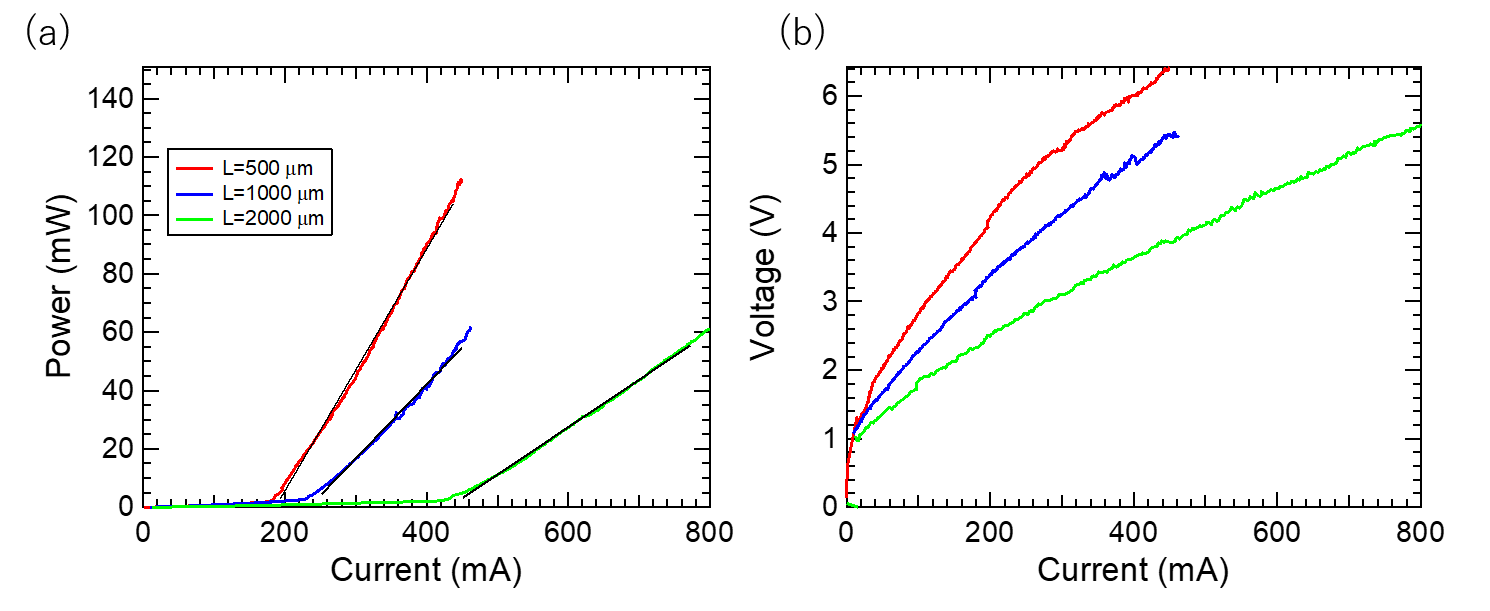
\includegraphics[width=15cm]{figure/fig_3_1_3QW_broadcontact_IL.png}
		\caption{3周期歪量子井戸ブロードコンタクトレーザーのILカーブとIVカーブ}
		\label{fig:fig_3_1_3QW_broacdcontact_IL}
\end{figure}

(a)を見ると各デバイスにおいて光出力強度が電流値を上げてくと増加していき、ある電流値を超えると発振が始まり発光強度が急激に増加することがわかる。その電流値を発振しているときのILカーブを直線フィッティングすることで求めた。フィッティング直線の$x$切片を発振閾値電流$I_{\rm{th}}$とした。またフィッティング直線の傾きを発振時のスロープ効率$\Delta P/\Delta I$とした。スロープ効率はフィッティングの傾きにデューティー比をかけ、共振器の両端面からの放出を考慮して2倍にして算出した。
典型的な値として、図\ref{fig:fig_3_1_3QW_broacdcontact_IL}(a)のILカーブの値を表\ref{table:table_3_1_3QW_broadcontact}に示す。表では
\begin{table}[h]
  \caption{3周期ブロードコンタクトレーザーの閾値電流}
  \label{table:table_3_1_3QW_broadcontact}
  \centering
  \begin{tabular}{ccc}
    \hline
    共振器長$L$(um)  & 閾値電流$I_{th}$ (mA)  & Slope 2$\Delta P/\Delta I$ (W/A) \\
    \hline \hline
     500& 187&  0.83  \\
    1000& 234& 0.51\\
    2000& 450&0.37\\
       \hline
  \end{tabular}
\end{table}



\ref{fig:fig_3_1_3QW_broacdcontact_IL}(b)を見ると各デバイスにおいて電流が流れ始めるのが1 V付近からでありダイオード特性が見られる。また共振器長$L$が長いほど同じ電流に対する電圧が低い。これは共振器長$L$に比例して電流が流れる面積が大きくなるためデバイスの抵抗値が小さくなっているためである。


次に様々なパッド幅に対して見積もった発振閾値電流$I_{\rm{th}}$の結果を図\ref{fig:fig_3_1_3QW_broadcontact_Ith}(a)に示す。発振閾値電流$I_{\rm{th}}$、横軸が電極パッド幅$w$である。\ref{fig:fig_3_1_3QW_broadcontact_Ith}(b)は発振時の発光効率$2 \Delta P/\Delta I$である。

図\ref{fig:fig_3_1_3QW_broadcontact_Ith}(a)を見ると、パッド幅$w$が50\si{ \micro\metre}より大きい領域では閾値電流$I_{\rm{th}}$はパッド幅$w$に対して線形に増加していることがわかる。一方パッド幅$w$が小さい領域では線形に変化していない。

この原因は電流がパッド幅$w$に対して無視できないほど広がってしまっているためだと考えられる。電流広がりについてはフィッティングから見積もった。詳しくは3.1.3節で述べる。

図\ref{fig:fig_3_1_3QW_broadcontact_Ith}(b)を見るとそれぞれの共振器長で概ね横ばいの値を持っている。$\Delta P/\Delta I$はパッド幅$w$に依存しないことがわかる。幅wは光の増幅を受ける方向とは関係がなく、直感と一致する。

\begin{figure}[h]
	\centering
	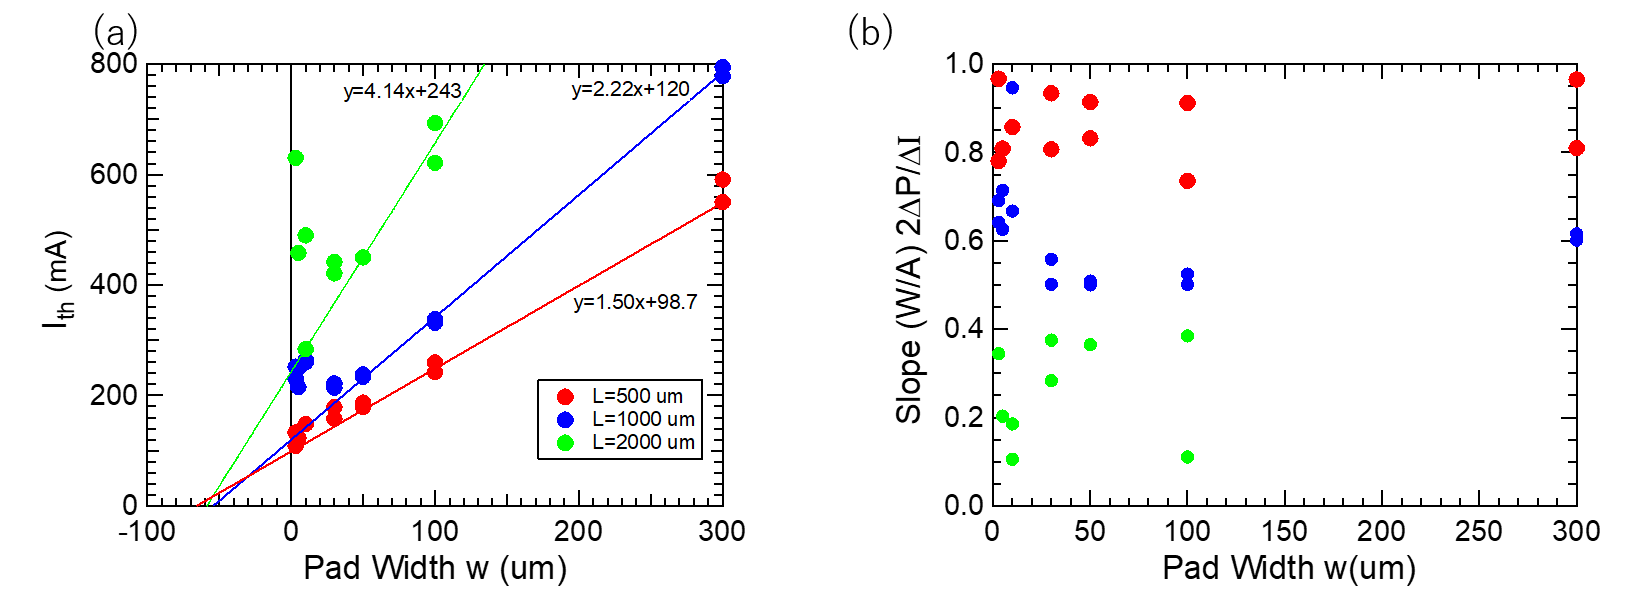
\includegraphics[width=15cm]{figure/fig_3_1_3QW_broadcontact_Ith.png}
		\caption{3周期歪量子井戸ブロードコンタクトレーザーの閾値電流と発光効率}
		\label{fig:fig_3_1_3QW_broadcontact_Ith}
\end{figure}
\clearpage
\subsection{10周期歪補償量子井戸ブロードコンタクトレーザー}%===============================
次に10周期歪補償量子井戸ブロードコンタクトレーザーについての結果を示す。図\ref{fig:fig_3_1_10QW_broadcontact_IL}(a)にILカーブ、(b)にIVカーブを示す。$w$=50 \si{\micro\metre}を代表としてプロットした。色分けは共振器長の違いを表す。電流は2 \si{\micro s}パルスを2 ms繰り返し周期で印可した。デューティー比は1:1000である。
\begin{figure}[h]
	\centering
	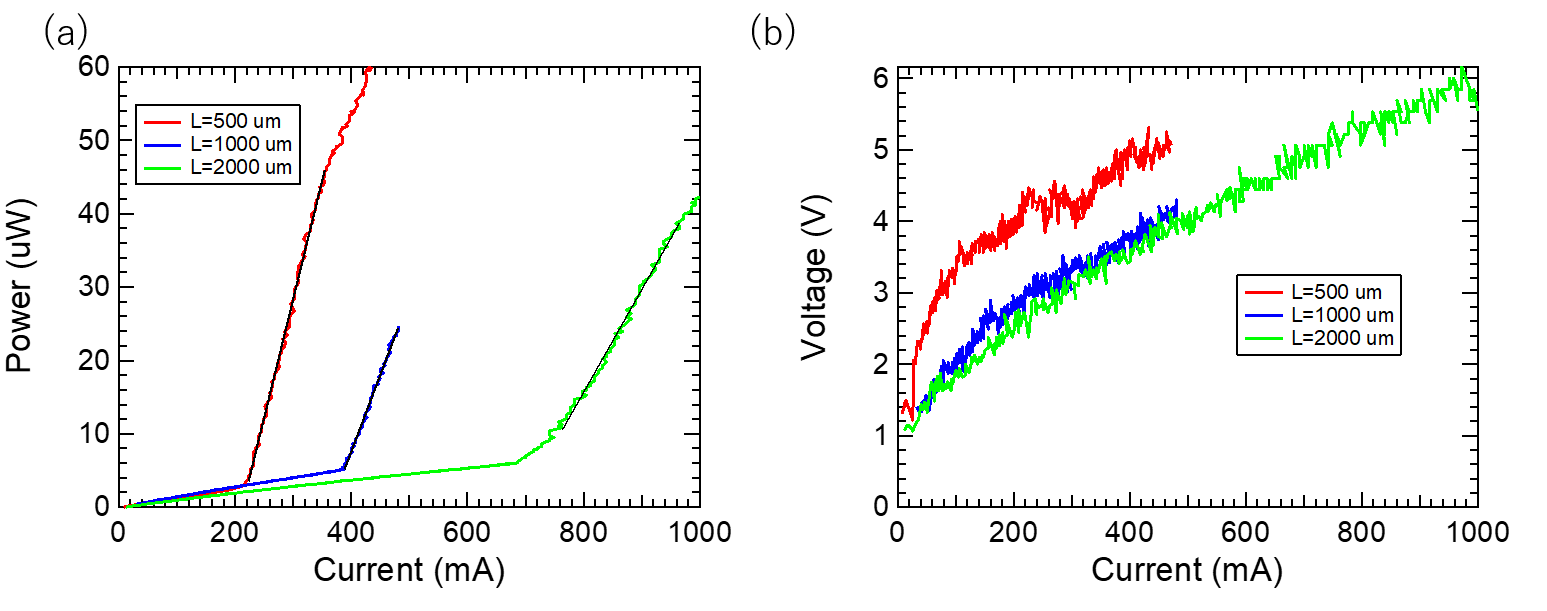
\includegraphics[width=15cm]{figure/fig_3_1_10QW_broadcontact_IL.png}
		\caption{10周期歪補償ブロードコンタクトレーザーのILカーブとIVカーブ}
		\label{fig:fig_3_1_10QW_broadcontact_IL}
\end{figure}

典型的な値として図
\ref{fig:fig_3_1_10QW_broadcontact_IL}(a)のILカーブフィッティング結果の値を表\ref{table:table_3_1_10QW_broadcontact}に示す。傾きはデューティー比1:1000と両端面からの発光を換算していることに注意されたい。
\begin{table}[h]
  \caption{10周期歪補償ブロードコンタクトレーザーの閾値電流}
  \label{table:table_3_1_10QW_broadcontact}
  \centering
  \begin{tabular}{ccc}
    \hline
    共振器長$L$(\si{\micro\metre})  & 閾値電流$I_{th}$ (mA)  & Slope 2$\Delta P/\Delta I$ (W/A) \\
    \hline \hline
     500& 212&  0.64  \\
    1000& 363& 0.42\\
    2000& 501&0.27\\
       \hline
  \end{tabular}
\end{table}

次に\adsp02{図}\ref{fig:fig_3_1_3QW_broadcontact_Ith} (a)に\ref{fig:fig_3_1_10QW_broadcontact_IL} (a)のILカーブの発振時の直線フィッティング結果から求めた閾値電流$I_{\rm{th}}$および(b)スロープ効率2 $\Delta P/\Delta I$をパッド幅$w$に対してプロットした。
\begin{figure}[h]
	\centering
	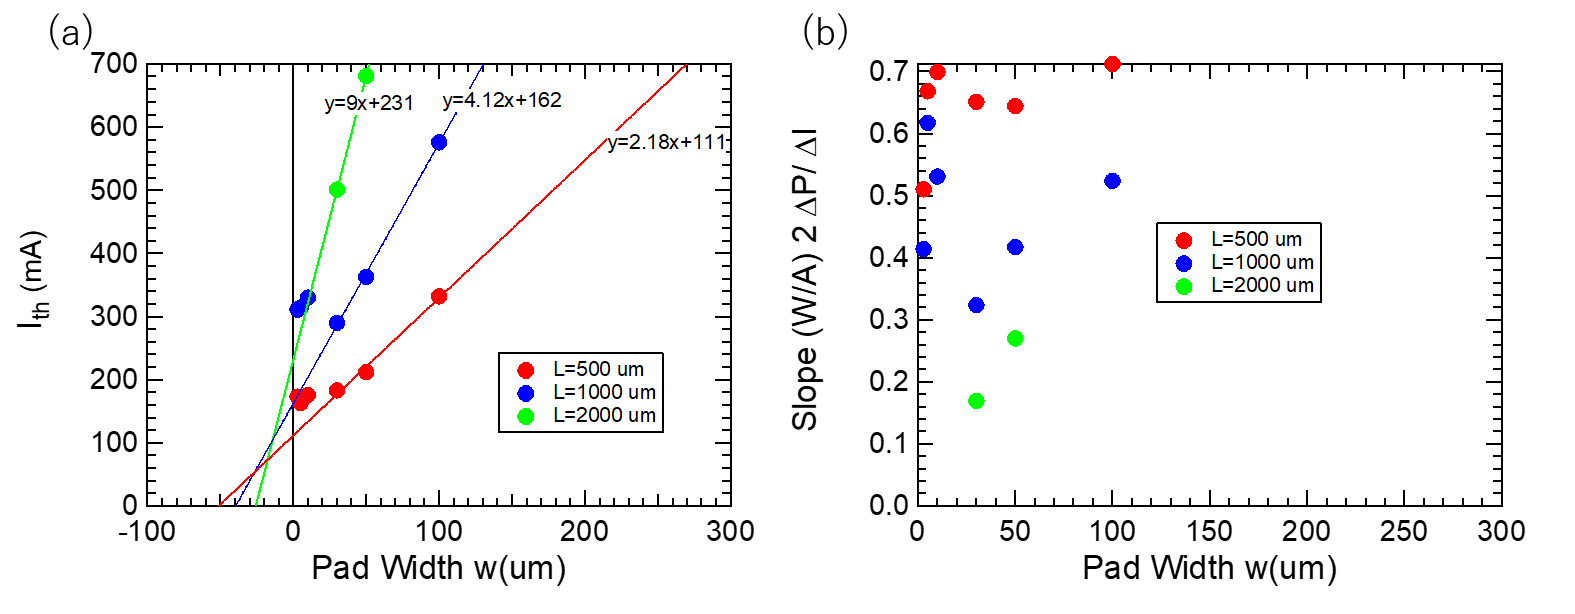
\includegraphics[width=15cm]{figure/fig_3_1_10QW_broadcontact_Ith.png}
		\caption{10MQWのIL結果}
		\label{fig:fig_3_1_10QW_broadcontact_Ith}
\end{figure}

\subsection{電流広がりに関する考察}%==================
3.1.1節と3.1.2節でILカーブから3周期歪量子井戸ブロードコンタクトレーザーと10周期歪補償ブロードコンタクトレーザーについて閾値電流$I_{\rm{th}}$を見積もった。閾値電流密度$J_{\rm{th}}$は半導体レーザーの性能を表す指標にもなるパラメータである。
レーザーの基本的な特性を知る上で閾値電流密度が大切なパラメータであるからである。発振閾値電流$I_{\rm{th}}$を電流が流れた面積で割ることで閾値電流密度$J_{\rm{th}}$が求まる。

通常閾値電流$I_{\rm{th}}$は電流を流す面積に比例して大きくなる。面積とは電極パッド幅$w$と共振器長$L$の積で表される。つまり$I_{\rm{th}}$は$w$に対して線形に増加するはずである。しかし図\ref{fig:fig_3_1_3QW_broacdcontact_IL} (a)や\ref{fig:fig_3_1_10QW_broadcontact_IL}(a) を見るとそうなっていない。そこで発振閾値電流$I_{\rm{th}}$が線形に増加する領域を直線フィッティングし、その直線の$x$切片を含めたパッド幅を有効的なパッド幅と考えて閾値電流密度を算出した。まずは有効パッド幅を見積もった。フィッティング関数の$x$切片の絶対値が実質的なパッド幅の増分$w'$である。その値を表\ref{table:table_3QW_broadcontact_w_eff}と表\ref{table:table_10QW_broadcontact_w_eff}に示した。
\begin{table}[h]
  \caption{3周期歪量子井戸ブロードコンタクトレーザーの電流広がり}
  \label{table:table_3QW_broadcontact_w_eff}
  \centering
  \begin{tabular}{cc}
    \hline
    共振器長$L$ (\si{\micro\metre})  & パッド幅の増分(電流の広がり) $w'$ (\si{\micro\metre})   \\
    \hline \hline
     500 & 65.8  \\
    1000  & 54.1 \\
    2000  & 58.7 \\ 
    \hline
  \end{tabular}
\end{table}

\begin{table}[h]
  \caption{10周期歪補償ブロードコンタクトレーザーの電流広がり}
  \label{table:table_10QW_broadcontact_w_eff}
  \centering
  \begin{tabular}{cc}
    \hline
    共振器長$L$ (\si{\micro\metre})  & パッド幅の増分(電流の広がり) $w'$ (\si{\micro\metre})   \\
    \hline \hline
     500 & 51.1  \\
    1000  & 39.5 \\
    2000  & 25.7 \\ 
    \hline
  \end{tabular}
\end{table}

3周期歪量子井戸レーザーでは58 \si{\micro\metre}から65 \si{\micro\metre}程度の広がりであることが見積もられた。10周期歪補償量子井戸レーザーでは25\si{ \micro\metre}から51\si{ \micro\metre}の広がりであると見積もられた。10周期歪補償値量子井戸レーザーでは値ののばらつきが大きく$L$=500 \si{\micro\metre}の$w'$と$L$=2000 \si{\micro\metre}の$w'$を比較すると2倍程度異なってしまっている。これは共振器の長い試料について、$w$が大きい試料に対しての実験結果がないため、$w'$の見積もりが小さくなってしまったためであると考えられる。さらに大電流を流して発振させる実験を行うことが必要である。


この表の値$w'$と閾値電流$I_{\rm{th}}$(mA)から式(\ref{eq:Jth})の関係を用いて閾値電流密度$J_{\rm{th}} \rm{(kA/cm^2)}$を算出した。
\begin{eqnarray}
J_{\rm{th}}=\dfrac{I_{\rm{th}}}{(w+w')L}
\label{eq:Jth}
\end{eqnarray}

その結果を示す。図\ref{fig:fig_3_1_3QW_broadcontact_Jth}に3周期歪量子井戸ブロードコンタクトレーザーの閾値電流密度、図\ref{fig:fig_3_1_10QW_broadcontact_Jth}に10周期歪補償量子井戸ブロードコンタクトレーザーの閾値電流密度をプロットした。

\begin{figure}[h]
	\centering
	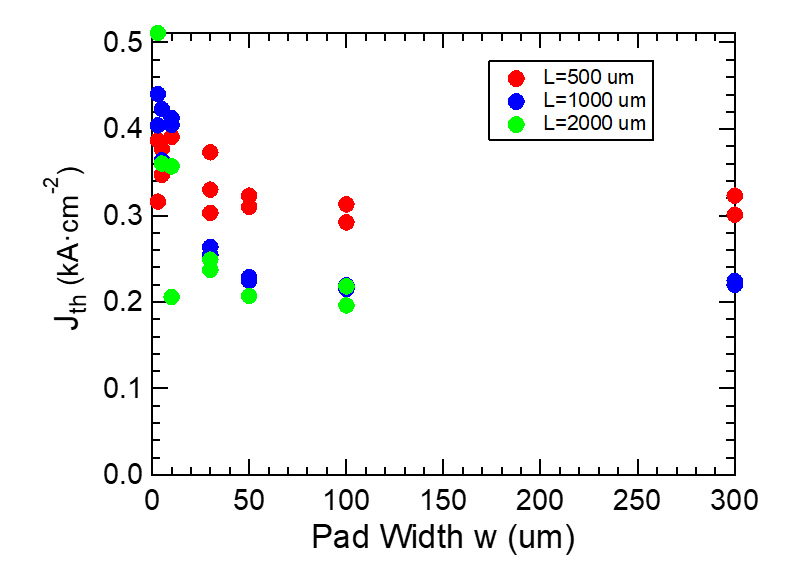
\includegraphics[width=10cm]{figure/fig_3_1_3QW_broadcontact_Jth.png}
		\caption{3周期歪量子井戸ブロードコンタクトレーザーの閾値電流密度}
		\label{fig:fig_3_1_3QW_broadcontact_Jth}
\end{figure}

\begin{figure}[ht]
	\centering
	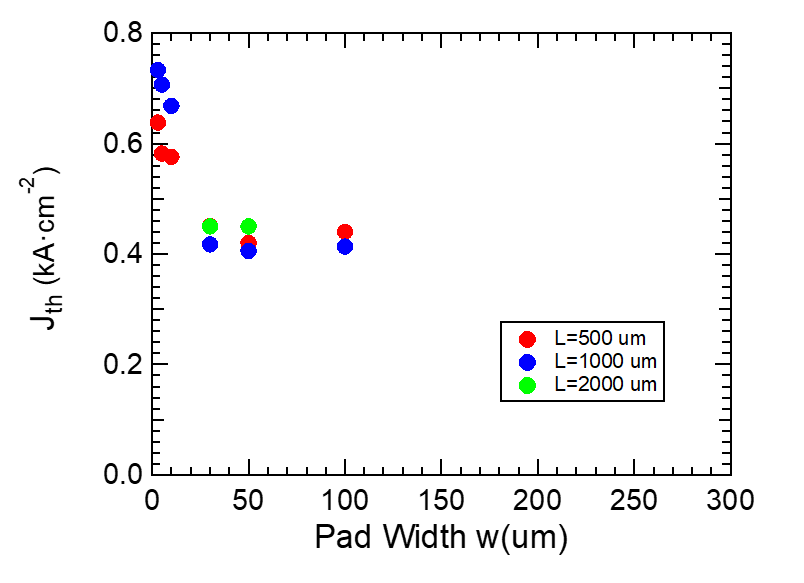
\includegraphics[width=10cm]{figure/fig_3_1_10QW_broadcontact_Jth.png}
		\caption{10周期歪補償量子井戸ブロードコンタクトレーザの閾値電流密度}
		\label{fig:fig_3_1_10QW_broadcontact_Jth}
\end{figure}
3周期歪量子井戸ブロードコンタクトレーザーでは$0.20\sim 0.35  \rm{ kA/cm^{2}}$、10周期歪補償ブロードコンタクトレーザーでは$0.40 \rm{ kA/cm^{2}}$程度と見積もられた。

3周期歪量子井戸ブロードコンタクトレーザーでは $w$が50 \si{\micro\metre}より大きい領域で、共振器長が長くなるほど閾値電流密度$J_{\rm{th}}$が小さくなることがわかる。
%これは共振器長が長くなるほどミラーロスに対する内部ロスが大きくなっていき、発振が起こりにくくなっているためである。

一方10周期歪補償量子井戸ブロードコンタクトレーザーではL=2000 \si{\micro\metre}の値が他の2つに比べて大きくなってしまっている。これは$w'$が小さく見積もられており、$J_{\rm{th}}$が大きく見積もられたためだと考えられる。$w'$の解析に用いたプロット点数が少ないことが原因である。

パッド幅$w$の広がり$w'$が数十\si{\micro\metre}とパッド幅に対して優位なほど広がっているという推察を得たが、この原因としてウエハの結晶構造が考えられる。図\ref{fig:fig_2_1_wafer_structure}のエピウエハ構造において活性層の上のSCH層の上に100 nm厚のp-$\rm{In_{0.485}Ga_{0.515}P}$層が挿入されている。このp-$\rm{In_{0.485}Ga_{0.515}P}$のバンドギャップは1.891 eVは上下を挟んでいるGaAsのバンドギャップ1.424 eVに比べて0.467 eV大きい。このバンドギャップの差によりキャリアが拡散され結晶面内へ広がってしまったと考えられる。

\clearpage
\subsection{外部量子効率、内部量子効率と吸収係数の計算}%=============
次にILカーブの発振時の傾きに相当するスロープ効率$\Delta P/\Delta I$から試料の内部微分量子効率$\eta_{i}$および吸収係数$\alpha$を算出した。まずはスロープ効率$2 \Delta P/\Delta I \rm{ (W/A)}$から外部微分量子効率$\eta_{\rm{d}}$を算出した。式({\ref{eq:eta_d})の関係を用いた。
\begin{eqnarray}
\eta_{\rm{d}}=\dfrac{e}{h\nu}2\dfrac{\Delta P}{\Delta I} 
\label{eq:eta_d}
\end{eqnarray}
eは電気素量、hはプランク定数、$\nu$は発振周波数であり、1050 nmとした。$\eta_{\rm{d}}$はキャリアの注入数に対する取り出せる光子の数の割合である。結果を図\ref{fig:fig_3_1_3QW_broadcontact_id}に示す。縦軸を$\eta_{\rm{d}}$横軸をパッド幅$w$としてプロットした。色分けが共振器長の違いを表している。$L$=500 \si{\micro\metre}では0.7程度、$L$=1000         \si{\micro\metre}では0.4程度、L=400 \si{\micro\metre}では0.3程度の値を持っている。
\begin{figure}[h]
	\centering
	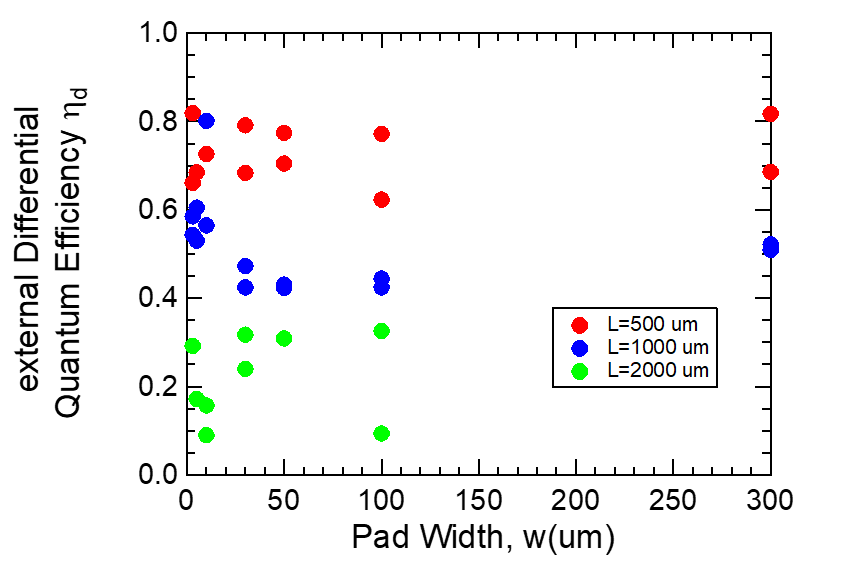
\includegraphics[width=10cm]{figure/fig_3_1_3QW_broadcontact_id.png}
	\caption{3周期歪量子井戸ブロードコンタクトレーザーの外部量子効率}
	\label{fig:fig_3_1_3QW_broadcontact_id}
\end{figure}

ここで$\eta_{d}$は共振器内での全発光にしめる共振器損失の割合であるから
\begin{eqnarray}
\eta_{d}=\eta_{int}\dfrac{\alpha_{m}}{\alpha_{int} +\alpha_{m}}
\end{eqnarray}
である。$\alpha_{int}$は共振器内の平均の内部損失、Rは共振器の端面での反射率、$\eta_{\rm{int}}$は内部微分量子効率である。
$\eta_{\rm{d}}$は共振器長$L$を用いて式(\ref{eq:eta_inverse})と書き表される。
\begin{eqnarray}
\dfrac{1}{\eta_{\rm{d}}}=\dfrac{\alpha_{\rm{int}}}{\rm{ln}(1/R)\eta_{int}}L+\dfrac{1}{\eta_{\rm{int}}}
\label{eq:eta_inverse}
\end{eqnarray}



RはGaAsの屈折率と空気の屈折率の差から0.32と仮定した。見積もった$\eta_{\rm{d}}$の逆数を共振器長に対してプロットし直線フィッティングを行なった。これを図\ref{fig:fig_3_1_3QW_broadcontact_id_inverse}に示す。横軸は共振器長$L$、縦軸に外部微分量子効率の逆数$1/\eta_{\rm{d}}$である。例としてパッド幅$w$=100 \si{\micro\metre}の結果を示す。式(\ref{eq:eta_inverse})よりこのフィッティング直線のy切片から内部量子効率$\eta_{\rm{int}}$を見積もると$\eta_{\rm{int}}$=0.96と計算できる。また、直線の傾きから内部損失$\alpha_{\rm{int}}$を見積もると$\alpha_{\rm{int}}$=11.8 /cmと計算できた。
\begin{figure}[h]
	\centering
	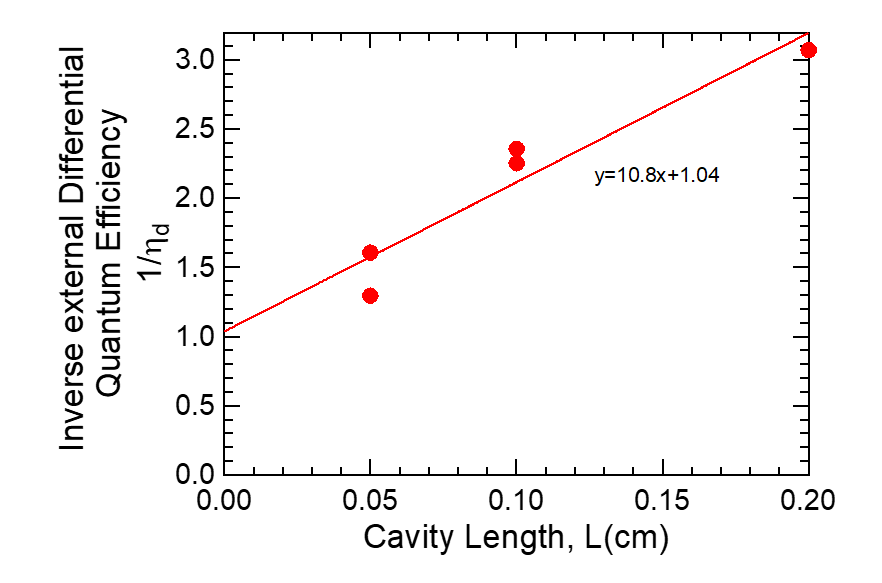
\includegraphics[width=10cm]{figure/fig_3_1_3QW_broadcontact_id_inverse.png}
	\caption{3周期歪量子井戸レーザーの外部量子効率の逆数}
	\label{fig:fig_3_1_3QW_broadcontact_id_inverse}
\end{figure}



\newpage

同様の解析を10周期歪補償量子井戸ブロードコンタクトレーザーの結果についても行った。図\ref{fig:fig_3_1_10QW_broadcontact_id}に外部微分量子効率、図\ref{fig:fig_3_1_10QW_broadcontact_id_inverse}\adsp02{に外部微分量子効率の逆数の共振器長依存性を示す。横軸は共振器長$L$、縦軸は外部微分量子効率の逆数$1/\eta_{\rm{d}}$である。}$w$=50\si{ \micro\metre} の結果を示している。10周期に関しては$\eta_{\rm{int}}$=0.94、$\alpha_{\rm{int}}$=18.0 (/cm)となった。
\begin{figure}[h]
	\centering
	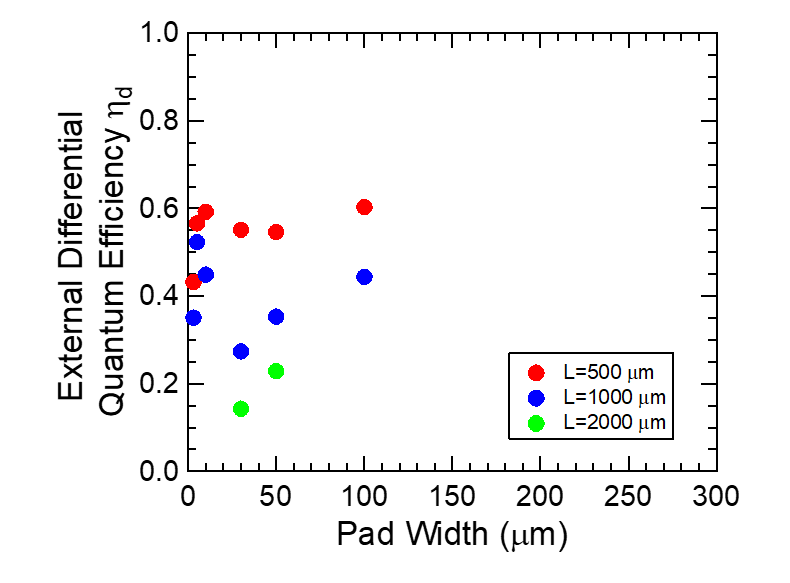
\includegraphics[width=10cm]{figure/fig_3_1_10QW_broadcontact_id.png}
	\caption{10QW外部量子効率}
	\label{fig:fig_3_1_10QW_broadcontact_id}
\end{figure}

\begin{figure}[h]
	\centering
	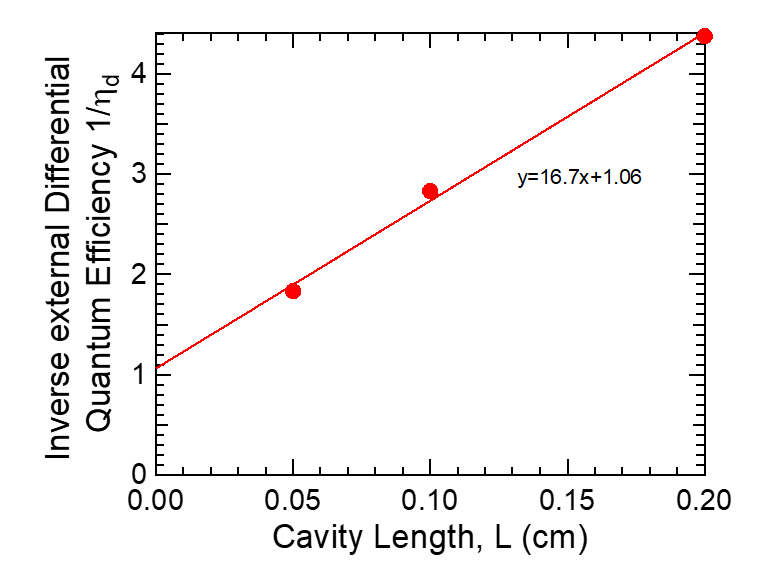
\includegraphics[width=10cm]{figure/fig_3_1_10QW_broadcontact_id_inverse.png}
	\caption{10QW外部量子効率の逆数}
	\label{fig:fig_3_1_10QW_broadcontact_id_inverse}
\end{figure}

\clearpage
\subsection{透明電流密度の見積もり}

次に透明電流密度$J_{0}$の見積もりを行った。共振器内の正味の利得$g_{\rm{net}}$は
\begin{eqnarray}
g_{\rm{net}}=\Gamma G-\alpha_{int}-\alpha_{m}
\label{eq:eta_j0}
\end{eqnarray}
と書ける。線形利得$G=g_{0}(J-J_{0})$を仮定すると閾値電流密度は
\begin{eqnarray}
J_{th}=J_{0}+\dfrac{\alpha_{int}}{\Gamma g_{0}}+\dfrac{1}{\Gamma g_{0}}\rm{ln}\left(\dfrac{1}{R}\right)\dfrac{1}{L}
\label{eq:j_th}
\end{eqnarray}
と書ける。この式にしたがうと$J_{\rm{th}}$は$1/L$に比例する。図\ref{fig:fig_3_1_3QW_broadcontact_j0}に$1/L$に対して$J_{\rm{th}}$をプロットした。色分けは共振器長を表す。
\begin{figure}[h]
	\centering
	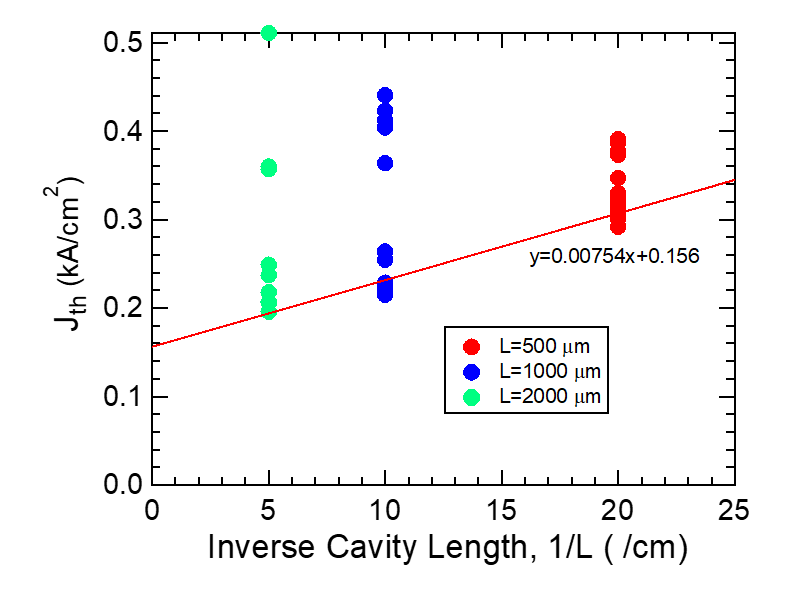
\includegraphics[width=10cm]{figure/fig_3_1_3QW_broadcontact_j0.png}
	\caption{3周期歪量子井戸ブロードコンタクトレーザーの透明電流密度の見積もり}
	\label{fig:fig_3_1_3QW_broadcontact_j0}
\end{figure}

図\ref{fig:fig_3_1_3QW_broadcontact_j0}のプロットのなかで、図\ref{fig:fig_3_1_3QW_broadcontact_Jth}の閾値電流密度をプロットした図において$J_{\rm{th}}$が一定となっている$w$が50 \si{\micro\metre}以上のプロットに対して線形フィッティングを行った。赤い直線がフィッティング直線である。フィッティング結果と式(\ref{eq:j_th})の関係を用いて$\Gamma g_{0}$と$J_{0}$を見積もると$\Gamma g_{0}=151 \rm{ kA^{-1}}$、$J_{0}=0.0782 \rm{kA/cm^{2}}$を得た。


10周期歪補償量子井戸ブロードコンタクトレーザーについても同様の解析を行った。図\ref{fig:fig_3_1_10QW_broadcontact_j0}に$J_{\rm{th}}$対$1/L$のプロットを示す。フィッティング結果から$\Gamma g_{0}$と$J_{0}$を見積もると$\Gamma g_{0}=558   \rm{kA^{-1}}$、$J_{0}=0.357 \rm{kA/cm^{2}}$を得た。
\begin{figure}[t]
	\centering
	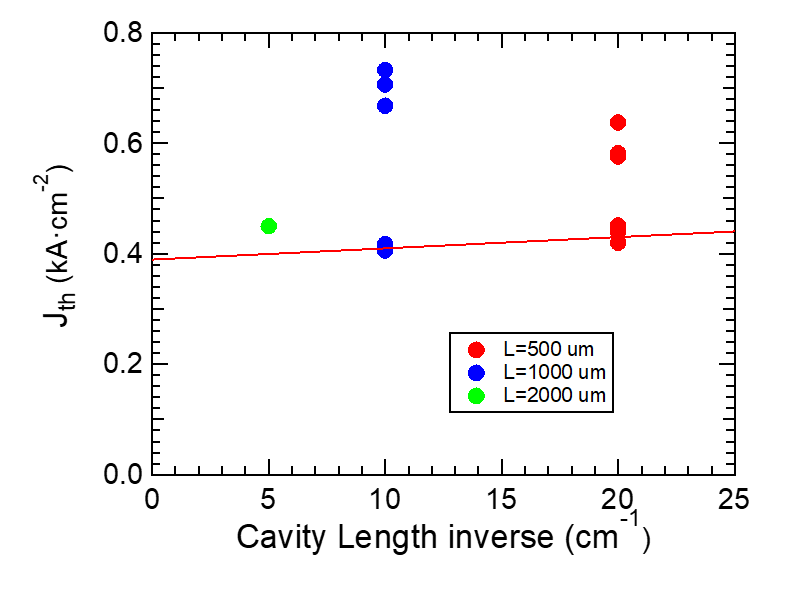
\includegraphics[width=10cm]{figure/fig_3_1_10QW_broadcontact_j0.png}
	\caption{10周期歪補償量子井戸ブロードコンタクトレーザーの透明電流密度の見積もり}
	\label{fig:fig_3_1_10QW_broadcontact_j0}
\end{figure}
\newpage
\subsection{ブロードコンタクトレーザーに対する電流注入実験のまとめと考察}

実験結果をまとめると3周期歪量子井戸ブロードコンタクトレーザーと10周期歪補償ブロードコンタクトレーザーに関して以下の表のようになる。
\begin{table}[h]
  \caption{ブロードコンタクトレーザーの結果まとめ}
  \label{table:table_I0}
  \centering
  \begin{tabular}{lcccc}
    \hline
    試料   &  内部損失$\alpha_{int} \rm{ /cm}$&内部量子効率$\eta_{int} $&透明電流密度 $J_{0} \rm{  kA/cm^2}$  &$\Gamma g_{0}$ /kA\\
    \hline \hline
     3周期 &   11.8 &0.96&0.0782 & 151\\
    10周期s  & 18.0 &0.94&0.357&558\\
    \hline
  \end{tabular}
\end{table}

内部損失は10周期試料の方が多くなった。
3周期試料と10周期試料を比較したとき透明電流密度は10周期試料が4.6倍となった。層数を増加させた効果が見えた。層数の比(活性層の厚さの比に等しい)が3.3倍であることを考えると式(\ref{eq:Mj0})で予想された透明電流密度の比よりも大きくなっている。また微分\adsp02{モード}利得係数$\Gamma g_{0}$の比は558/151=3.7となった。
モード利得$\Gamma G=\Gamma g_{0}(J-J_{0})$を図\ref{fig:fig_3_1_broadcontact_modal_gain}にプロットした。

\begin{figure}[t]
	\centering
	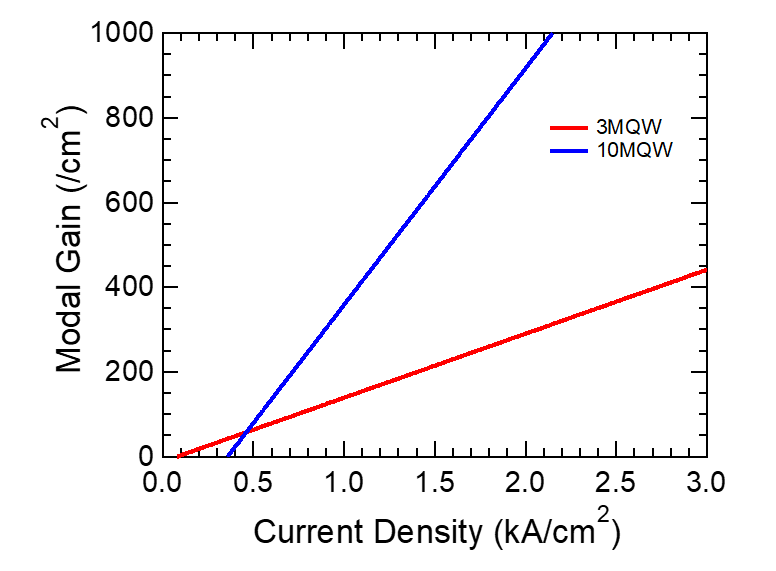
\includegraphics[width=10cm]{figure/fig_3_1_broadcontact_modal_gain.png}
	\caption{モード利得の電流密度依存性}
	\label{fig:fig_3_1_broadcontact_modal_gain}
\end{figure}
これを見ると0.5$ \rm{kA/cm^2}$ 以下では層数の少ない3周期試料の方がモード利得は大きく、それ以降では10周期試料の方が高いモード利得が得られることがわかる。この振る舞いは図	\ref{fig:fig_gain_mode}の理論計算により求められたモード利得の振る舞いと一致している。
\clearpage
\section{リッジ導波路型レーザーに関する実験結果}%===================
ブロードコンタクトレーザーを用い、半導体レーザーの基本的な特性を調べた。次に完成したデバイスとしてのリッジ導波路型レーザーに短パルス電流を印可し、利得スイッチング動作を行った。
\subsection{定常電流の結果}

利得スイッチング動作を行う前にまずは発振するか確かめること、および閾値電流を見積もることを目的として定常電流による標準的なデバイス評価実験を行なった。方法はブロードコンタクトレーザーの評価測定と同じである。
\subsubsection{3周期歪量子井戸リッジ導波路型レーザーの結果}
まずは3周期歪量子井戸リッジ導波路型レーザーの結果を示す。2 \si{\micro s}パルスを2 ms周期で印可した。デューティー比は1:1000である。
まずは3周期歪量子井戸リッジ導波路型レーザーの結果を図\ref{fig:fig_3_2_3QW_ridge_IL}に示す。図\ref{fig:fig_3_2_3QW_ridge_IL}(a)はILカーブ、(b)はIVカーブである。色分けは共振器長$L$の違いを表す。

\begin{figure}[h]
	\centering
	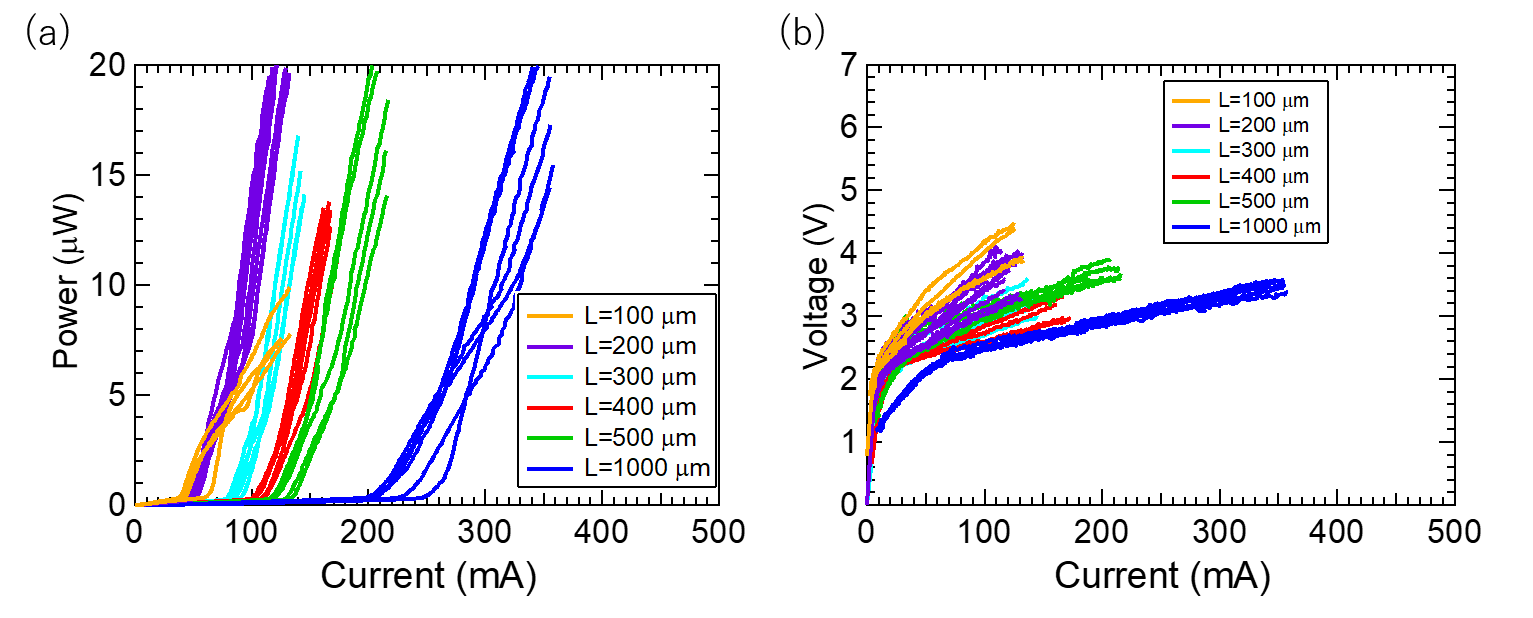
\includegraphics[width=15cm]{figure/fig_3_2_3QW_ridge_IL.png}
		\caption{3周期歪量子井戸リッジ導波路型レーザーのILカーブおよびIVカーブ}
		\label{fig:fig_3_2_3QW_ridge_IL}
\end{figure}


次にILカーブから見積もった閾値電流$I_{\rm{th}}$、$J_{\rm{th}}$と閾値電流密度を図\ref{fig:fig_3_2_3QW_ridge_Ith}に示す。図中の丸プロットが閾値電流$I_{\rm{th}}$であり左の軸に対してのプロットした。十字プロットは閾値電流を共振器長とリッジ幅の積で割った値の閾値電流密度$J_{\rm{th}}$であり右の軸に対してのプロットである。横軸は共振器長である。色分けはリッジ幅の違いを表している。紫色がリッジ幅1.5 \si{\micro\metre}、黄色が2.5 \si{\micro\metre}である。

これを見ると閾値電流は共振器長に対して概ね線形に増加しており\delsp02{最短では}\adsp02{最小の閾値電流は$L$=100 \si{\micro\metre}のときであり}50 mA程度となっている。またリッジ幅を1.5 \si{\micro\metre} 、 2.5 \si{\micro\metre}と変えても閾値電流に差が見られていない。これはブロードコンタクトレーザーで示唆されたように電流が広がってしまい有効的なリッジ幅は実際のリッジ幅よりも広いと考えられる。したがって閾値電流密度を見積もることは難しい。

閾値電流密度は$L$が300 \si{\micro\metre}より大きい共振器長において概ね横ばいとなっており10から20 $\rm{kA/cm^2}$の値を持っている。またリッジ幅による差異は単に同程度の閾値電流を異なるリッジ幅で割ったためである。


\begin{figure}[h]
	\centering
	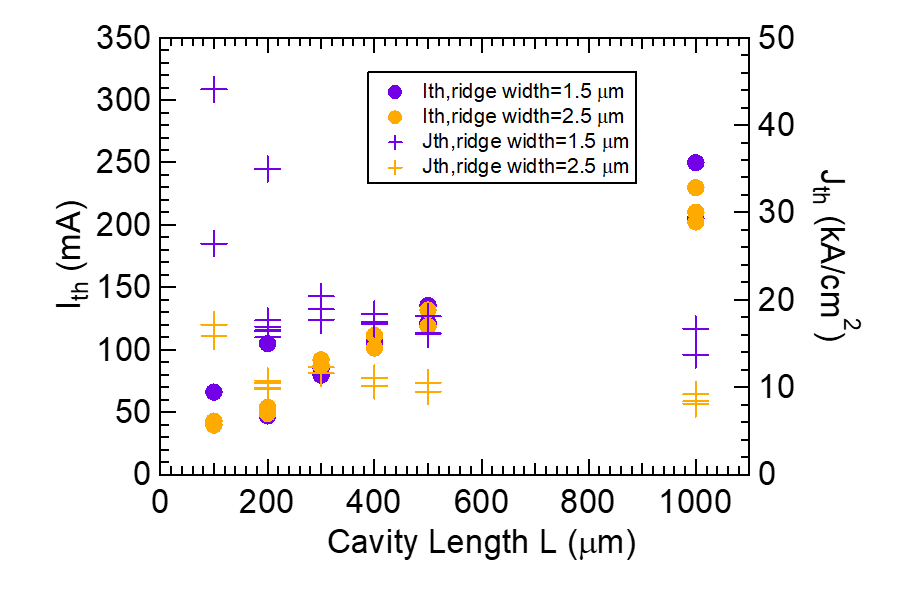
\includegraphics[width=10cm]{figure/fig_3_2_3QW_ridge_Ith.png}
		\caption{3周期歪量子井戸リッジ導波路型レーザーの$I_{\rm{th}}$、$J_{\rm{th}}$}
		\label{fig:fig_3_2_3QW_ridge_Ith}
\end{figure}
次にILカーブの発振領域の発光効率$2 \Delta P/\Delta I$および外部微分量子効率$\eta_{\rm{d}}$を共振器長に対してプロットした結果を図\ref{fig:fig_3_2_3QW_ridge_slope}に示す。発光効率$2 \Delta P/\Delta I$は0.03から0.87 W/A の値となった。また外部微分量子効率は0.026から0.87の値を持っている。
%L=100だけ低くなる原因ある?
\begin{figure}[h]
	\centering
	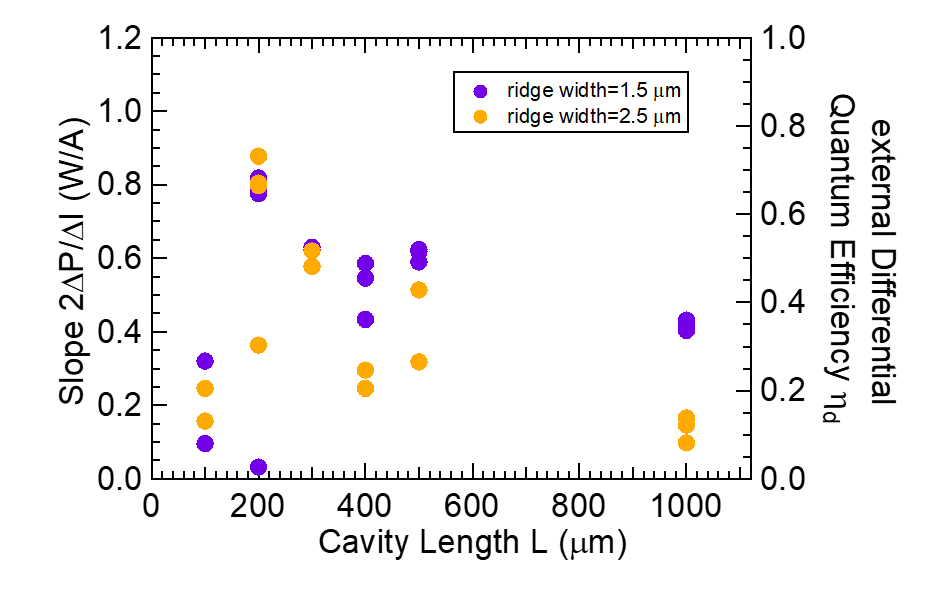
\includegraphics[width=10cm]{figure/fig_3_2_3QW_ridge_slope.png}
		\caption{3周期歪量子井戸リッジ導波路型レーザーのスロープおよび外部微分量子効率}
		\label{fig:fig_3_2_3QW_ridge_slope}
\end{figure}

\clearpage
\subsubsection{10周期歪補償量子井戸リッジ導波路レーザー}
次に10周期歪補償量子井戸リッジ導波路レーザーの結果を示す。図\ref{fig:fig_3_2_10QW_ridge_IL}(a)にILカーブ、(b)にIVカーブを示す。

\ref{fig:fig_3_2_10QW_ridge_IL}(a)を見るとそれぞれの共振器長において発振したことがわかる。$L$= 400\si{\micro\metre}の赤い線を見ると$I$= 200mA付近からどの試料においても発光量が下がってきている。
\begin{figure}[h]
	\centering
	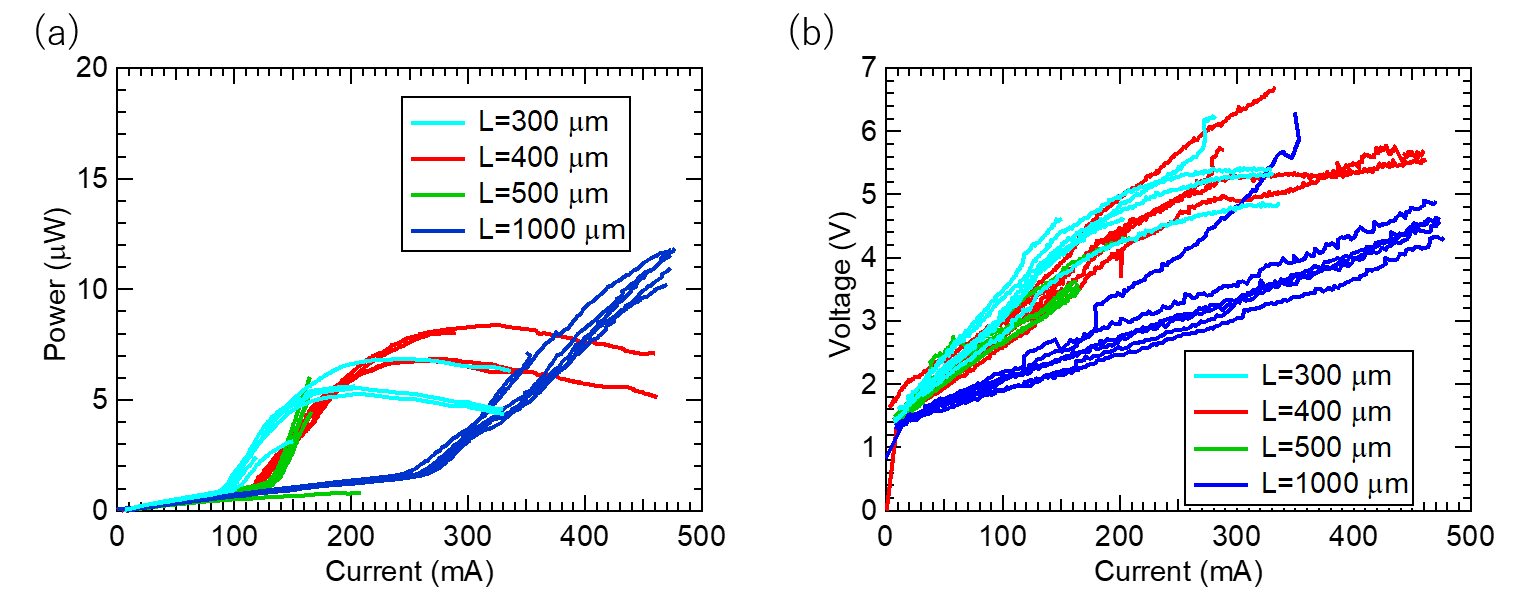
\includegraphics[width=15cm]{figure/fig_3_2_10QW_ridge_IL.png}
		\caption{10周期歪量子井戸リッジ導波路型レーザーのILカーブおよびIVカーブ}
		\label{fig:fig_3_2_10QW_ridge_IL}
\end{figure}
次にILカーブから閾値電流$I_{\rm{th}}$と閾値電流密度$J_{\rm{th}}$を算出した。その結果を図\ref{fig:fig_3_2_10QW_ridge_Ith}に示す。閾値電流は共振器長に対して線形に増加しており最小で90 mA程度となった。色分けはリッジ幅の違いを表すが、3周期試料と同様に閾値電流においてリッジ幅の際は見られない。閾値電流密度は10から20 $\rm{kA/cm^{2}}$程度となったが電流広がりの影響を考えていないため正しく見積もることはできていない。
\begin{figure}[h]
	\centering
	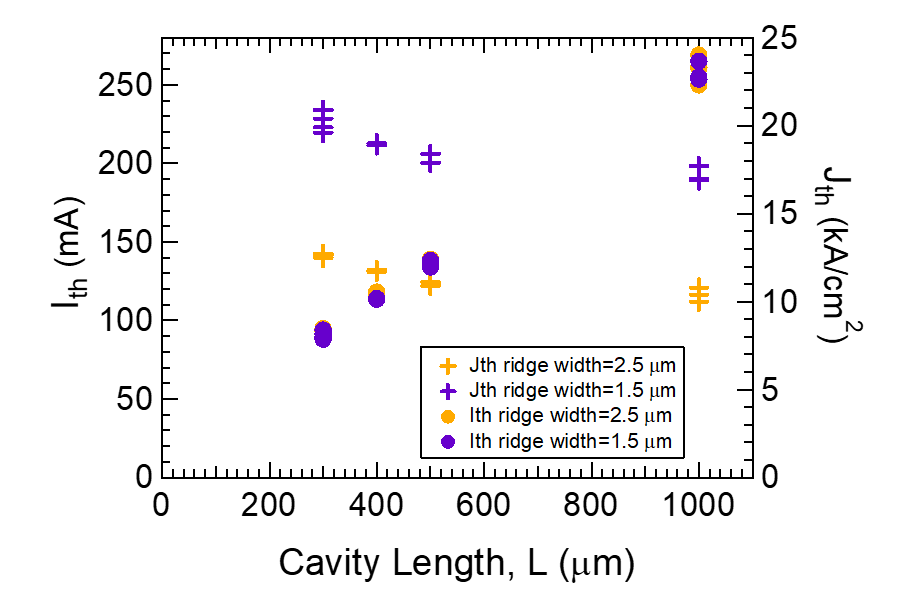
\includegraphics[width=10cm]{figure/fig_3_2_10QW_ridge_Ith.png}
		\caption{10周期歪補償量子井戸リッジ導波路型レーザーの閾値電流と閾値電流密度}
		\label{fig:fig_3_2_10QW_ridge_Ith}
\end{figure}
ILカーブの発振時の傾きから見積もったスロープ効率$2\Delta P/\Delta I$および外部微分量子効率$\eta_{\rm{d}}$を図\ref{fig:fig_3_2_10QW_ridge_slope}に示す。$\eta_{d}$は発振波長1030 nmとして計算した。通常$\eta_{d}$は共振器長に対しては減少するはずであるが(式(\ref{eq:eta_inverse}による))、 $L$=300 \si{\micro\metre},  400  \si{\micro\metre}では$L$の増加に対して減少が見られない。図\ref{fig:fig_3_2_10QW_ridge_IL}(a)を見てもこの2種類の共振器長に関してはILカーブが曲がり発光量が減少していることがわかる。


\begin{figure}[ht]
	\centering
	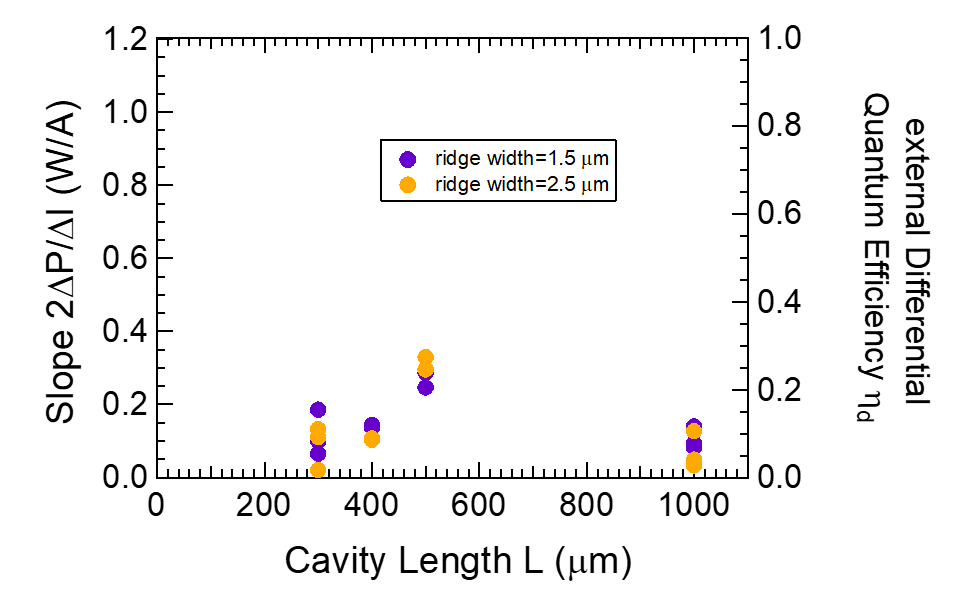
\includegraphics[width=10cm]{figure/fig_3_2_10QW_ridge_slope.png}
		\caption{10周期歪補償量子井戸リッジ導波路型レーザーのスロープおよび外部微分量子効率}
		\label{fig:fig_3_2_10QW_ridge_slope}
\end{figure}

\subsection{リッジ導波路型レーザーへの定常電流注入実験の結果まとめ}
\subsubsection{3周期歪量子井戸試料と10周期歪補償量子井戸試料の比較}
3周期試料と10周期試料を比較すると閾値電流は同程度外部微分量子効率は\delsp02{1}\adsp02{3}周期試料の方が高いという結果を得た。

また発振する前の発光強度を見てみると10周期試料の方が大きい\delsp02{ことがわかる}。自然放出光の強度が10周期試料の方が大きいことがわかる。
\subsubsection{10周期歪補償リッジ導波路型レーザーのILカーブのドループについて}
ここで10周期歪補償量子井戸リッジ導波路型レーザーのILカーブにおいて観測された発光の飽和および\adsp02{ドループ(注入増に対する発光強度減)}\delsp02{減衰}について述べる。このような発光量の飽和現象の原因としてはデバイスの温度上昇やそれに伴う吸収係数の増大、利得飽和(レート方程式における$\epsilon$の効果)、反射端面の光学損傷、空間のホールバーニング効果などが挙げられる。

これらの中から実験的に原因を特定するためには、発光の遠視野像を撮像することや活性層ではなくp側のGaAs層での発光強度を観察することが良いと考えられる。特に先の実験からInGaP層が障壁の役割をしていると想像されているため、その上下のGaAs層で発光が起こっている可能性が高く、その注入電流に対するGaAs発光強度を測定することができればデバイス内部のキャリアの分布が決められるのではないかと考えられる。
%ここでキャリアの再結合過程を考えると式(\ref{eq:tau_r})の非発光再結合には
%\begin{equation}
%\dfrac{1}{\tau_{nr}}(n)=A_{1}+A_{2}n+A_{3}n^2
%\end{equation}
%とキャリア密度nの二乗に比例するようなオージェ再結合が起こることが知られている。
%ILカーブを見るとこの中で共振器長に対して依存性が
%空間ホールバーニングはモードを確認すれは良い,filamentation(繊維化)

\clearpage
\subsection{短パルス電流注入の結果}

次にリッジ導波路型レーザーに関して1 ns矩形波電気パルスを印可し電流注入利得スイッチング実験を行った。そのILカーブと時間波形を示す。
\subsection{ILカーブ}
短パルス駆動時のILカーブを示す。その際電流に換算することが困難であったため、横軸はパルスの電圧である。
\subsubsection{3周期歪量子井戸レーザーのILカーブ}
図\ref{fig:fig_3_2_3QW_ridge_GS_power}に3周期歪量子井戸リッジ導波路型レーザーの短パルス駆動時のILカーブを示す。励起パルスのパルス幅は1 nsである。3つの異なる共振器長において発振が確認できた。共振器長はL=100 \si{\micro\metre}、200 \si{\micro\metre}、300 \si{\micro\metre}である。試料はレーザーバーの状態のものを用いた。\adsp02{1 cm程度芯線をむき出しにした同軸ケーブルを試料から5 mm程度の場所に固定し、芯線とp電極を金線でワイヤリングを行った。作業の都合上$L$=200 \si{\micro\metre}に関してワイヤーの長さは他の試料よりも2 mm程度長くなった。同軸ケーブルののグランド側は試料が乗っている約2 cm角の銅板に密着させた。}\delsp02{むき出しにしたものを試料の近く1cm程度($L$=200 umは3 cm程度と遠い)まで近づけ、芯線とレーザーの電極を金線でワイヤリングを行った。したがって回路全体の特性}インピーダンスにマッチ\delsp02{しているか定かでない。}\adsp02{のためのマッチング抵抗の付加などを行っていない。}

\begin{figure}[h]
	\centering
	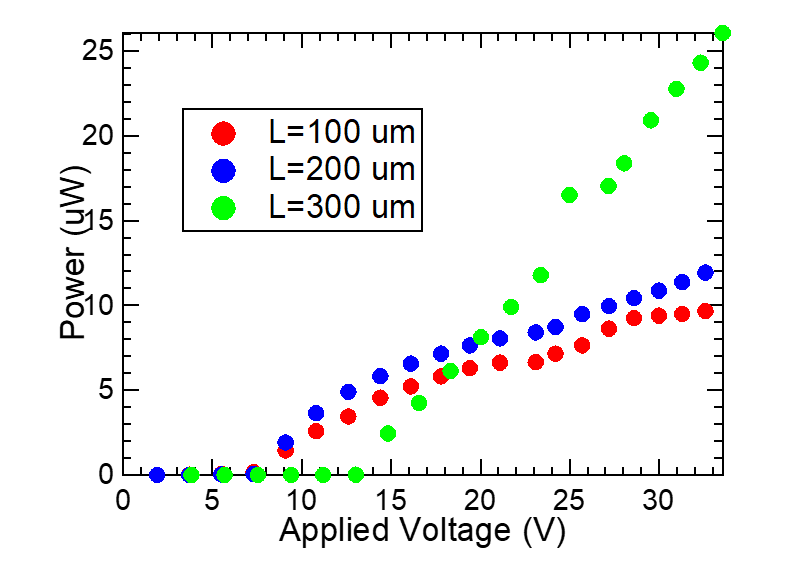
\includegraphics[width=10cm]{figure/fig_3_2_3QW_ridge_GS_power.png}
		\caption{3周期歪量子井戸 短パルス駆動時のILカーブ}
		\label{fig:fig_3_2_3QW_ridge_GS_power}
\end{figure}


\newpage
\subsubsection{10周期歪補償量子井戸レーザーのILカーブ}
次に図\ref{fig:fig_3_2_10QW_ridge_GS_power}に10周期歪補償量子井戸リッジ導波路型レーザーの短パルス駆動時のILカーブを示す。共振器長は$L$=300 \si{\micro\metre}、400 \si{\micro\metre}、500 \si{\micro\metre}である。10周期試料は全て\adsp02{1つずつに分離、チップ化しTO-}CANタイプの\adsp02{のキャリアにマウントした}試料である。\delsp02{インピーダンスマッチが取れており、高速電気パルスが形状を崩さず入っているとみなしている。}\adsp02{TO-CANのp側の足をSMAコネクタの芯線とAuSnはんだを用いて導通を取り(距離は0 )、n側の足は5 mm程度の金線空中配線によりSMAコネクタのグランドと繋げた。}

図\ref{fig:fig_3_2_10QW_ridge_GS_power}を見ると3つの異なる共振器長の試料に対して発振が確認できた。
%発振閾値書くか?
\begin{figure}[h]
	\centering
	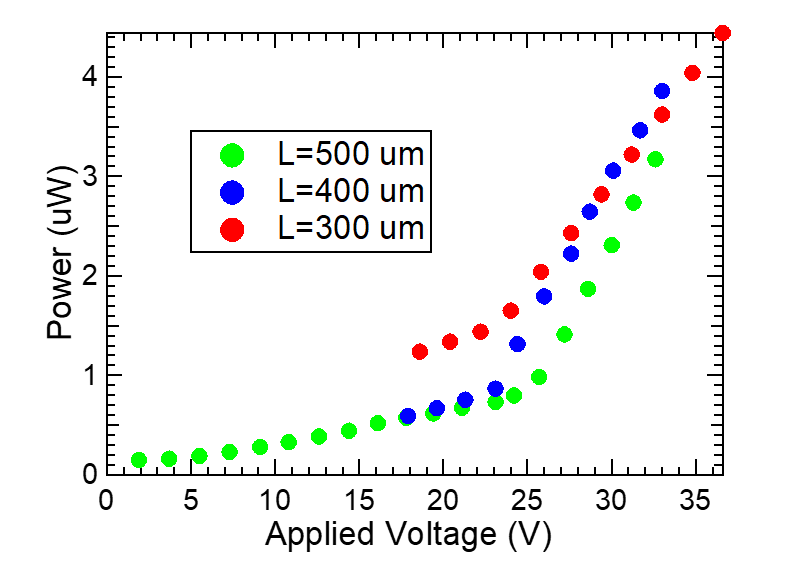
\includegraphics[width=10cm]{figure/fig_3_2_10QW_ridge_GS_power.png}
		\caption{10歪補償量子井戸リッジ導波路型レーザーの短パルス駆動時のILカーブ}
		\label{fig:fig_3_2_10QW_ridge_GS_power}
\end{figure}
\clearpage
\subsection{3周期歪量子井戸試料の利得スイッチング動作}%===============================
次にフォトダイオードで光を検出し高速オシロスコープで電気信号をモニタした時間波形を示す。図\ref{fig:fig_3_2_3QW_ridge_L100_GS}(a)に3周期歪量子井戸レーザーの共振器長$L$=100 \si{\micro\metre}試料の利得スイッチング動作の時間波形を示す。励起強度を変えた実験結果を示す。図\ref{fig:fig_3_2_3QW_ridge_L100_GS}(b)には強度を規格化したプロットをしめす。(a)を見ると励起強度を\delsp02{あげる}\adsp02{増大させる}にしたがってピーク強度が高くなって行くが途中で頭打ちになっている。(b)を見ると21 V程度までは励起強度の増加につれて立ち上がりが早くなっているがそれより強励起ではわずかに遅くなって\delsp02{いって}いる。
\begin{figure}[h]
	\centering
	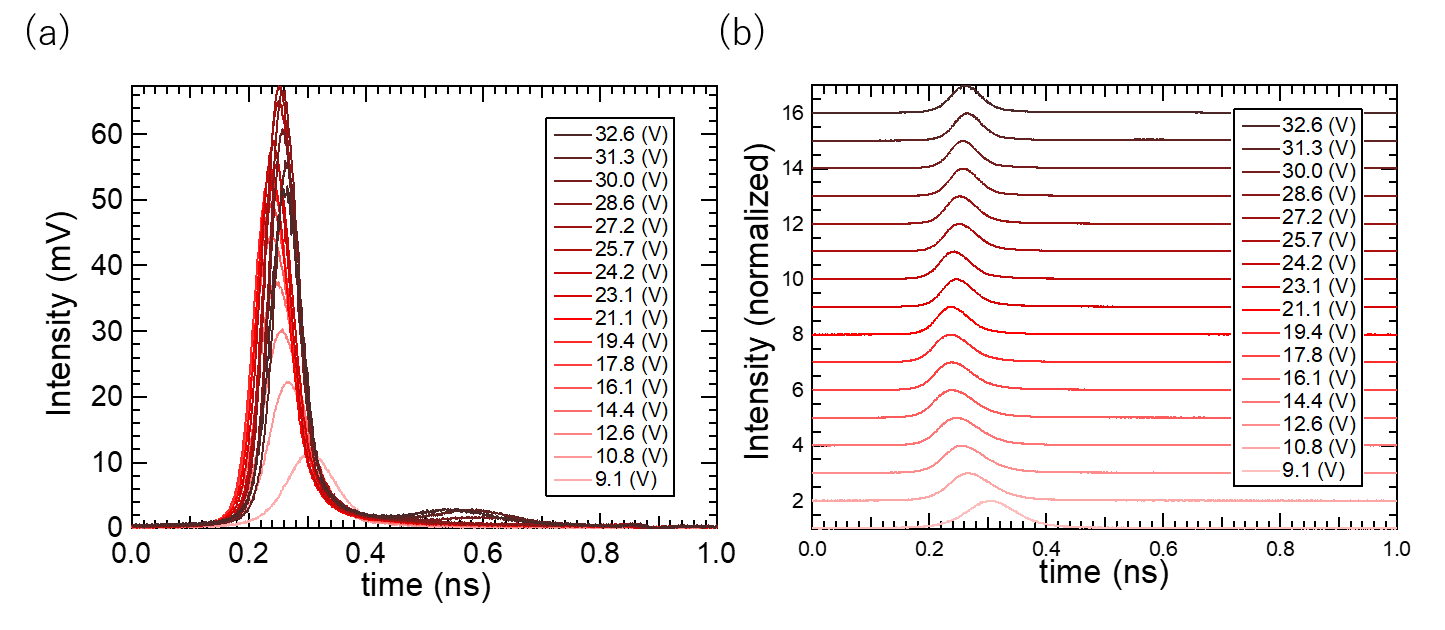
\includegraphics[width=15cm]{figure/fig_3_2_3QW_ridge_L100_GS.png}
		\caption{3周期歪量子井戸レーザー $L$=100 \si{\micro\metre} の利得スイッチング光パルスの時間波形}
		\label{fig:fig_3_2_3QW_ridge_L100_GS}
\end{figure}


図\ref{fig:fig_3_2_3QW_ridge_L200_GS}には$L$=200 \si{\micro\metre}試料の結果を示す。(a)を見ると励起強度を増加させるにしたがって1つめの光パルス強度は途中までは増加するもののあるところから減衰することがわかる。また途中から第2の光パルスが見られる。電流注入利得スイッチングに特有の緩和振動である。(b)を見ると光パルスの立ち上がりは励起強度とともに遅くなっていく様子が見られる。
%2番目のパルスの地上がり時間からなんかわからんの?それが緩和振動なのかどうか


\begin{figure}[h]
	\centering
	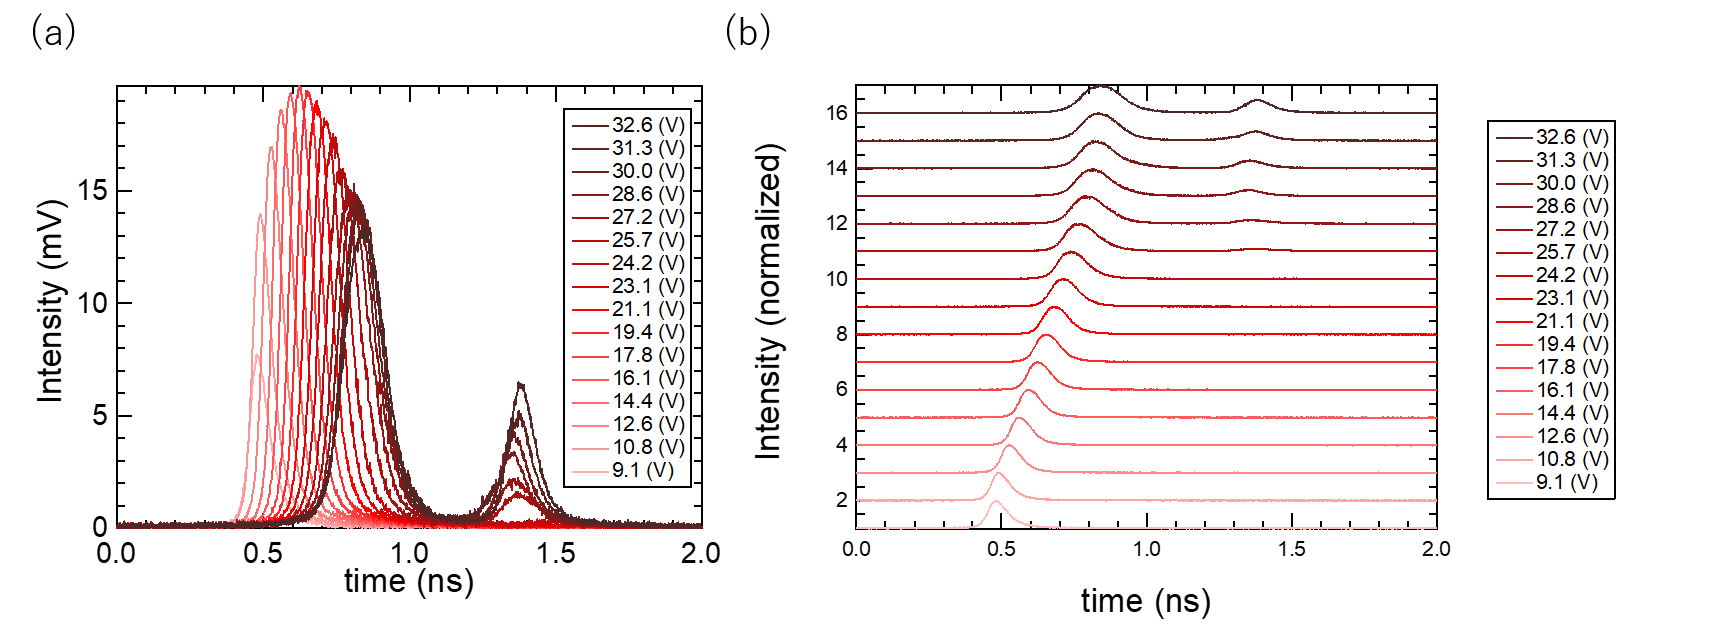
\includegraphics[width=15cm]{figure/fig_3_2_3QW_ridge_L200_GS.png}
		\caption{3周期歪量子井戸レーザー $L$=200 \si{\micro\metre} の利得スイッチング光パルスの時間波形}
		\label{fig:fig_3_2_3QW_ridge_L200_GS}
\end{figure}



図\ref{fig:fig_3_2_3QW_ridge_L300_GS}には$L$=300 \si{\micro\metre}試料の結果を示す。(a)の青い矢印は第1ピーク\delsp02{の場所}\adsp02{位置}の移り変わりを表している。(a)を見ると第1パルスは一度極大値を持ったのち遅くなっている。また途中から第2パルスが見られるようになり第2パルスの方が第1パルスよりも大きくなる場合が見られる。(b)を見ると励起強度を上げていくと20.0 Vまではシングルパルスであることがわかる。20.0 Vで立ち上がり時間が遅くなり、それ以上の励起強度では複数のピークを持ったまま立ち上がり時間が早くなっていく様子がわかる。長い電流パルスの影響による緩和振動であると考えられる。
\begin{figure}[h]
	\centering
	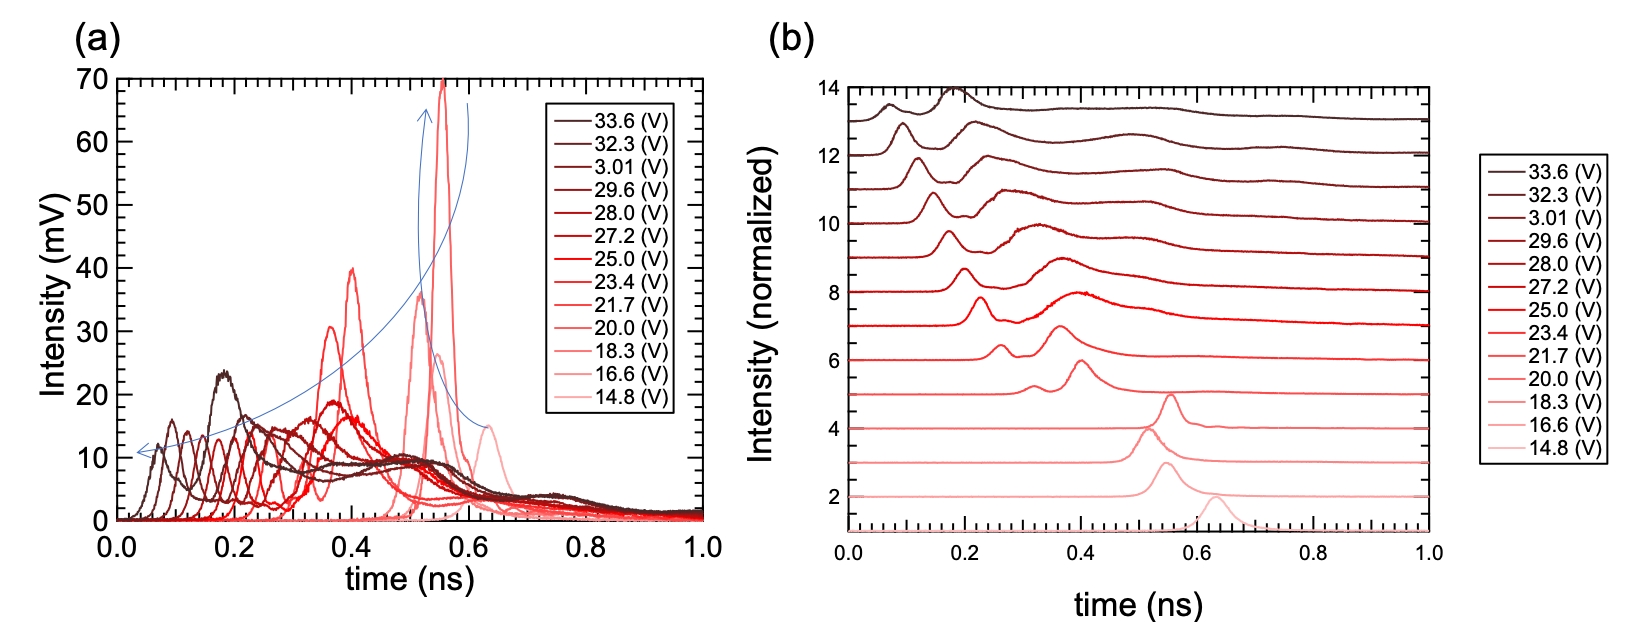
\includegraphics[width=15cm]{figure/fig_3_2_3QW_ridge_L300_GS.png}
		\caption{3周期歪量子井戸レーザー$ L$=300 \si{\micro\metre} の利得スイッチング光パルスの時間波形}
		\label{fig:fig_3_2_3QW_ridge_L300_GS}
\end{figure}


$L$=100 \si{\micro\metre}、200 \si{\micro\metre}、$L$=300 \si{\micro\metre}で見られた立ち上がりが遅くなる現象およびは通常の利得スイッチングの動作とは異なる。その原因は励起パルスが正常に印加されていないためではないかと考えられる。どの試料も配線する際の金線の長さが長く\delsp02{、インピーダンスが大きくなってしまったため、}短い電圧パルスが形を保てなかったと同時に励起強度も低くなってしまったと推測できる。
\subsubsection{3周期歪量子井戸リッジ導波路型レーザーの利得スイッチング実験結果まとめ}
ここで利得スイッチング光パルスの第1パルスのパルス幅を示す。ここでパルス幅は半値全幅FWHMとしている。また光の検出に用いた25 GHzフォトダイオードによるパルス広がりを考慮してdeconvolutionを行った結果を示す。

図\ref{fig:fig_3_2_3QW_ridge_GS_FWHM}に3周期歪量子井戸リッジ導波路型レーザーの利得スイッチング光パルスのパルス幅を示す。縦軸FWHM、横軸が励起強度である。色分けは共振器長の違いを表す。

$L$=100 \si{\micro\metre}、200 \si{\micro\metre}では励起強度を上げるとパルス幅が長くなっている。\delsp02{これはインピーダンスマッチが取れていない事による電気パルスの変形だと考えられる。}$L$=300 \si{\micro\metre}ではパルス幅30 ps程度の値を示し。飽和が起こっている。最短パルス幅はL=300 \si{\micro m}、23.4 V印加で28.9 psであった。
\begin{figure}[ht]
	\centering
	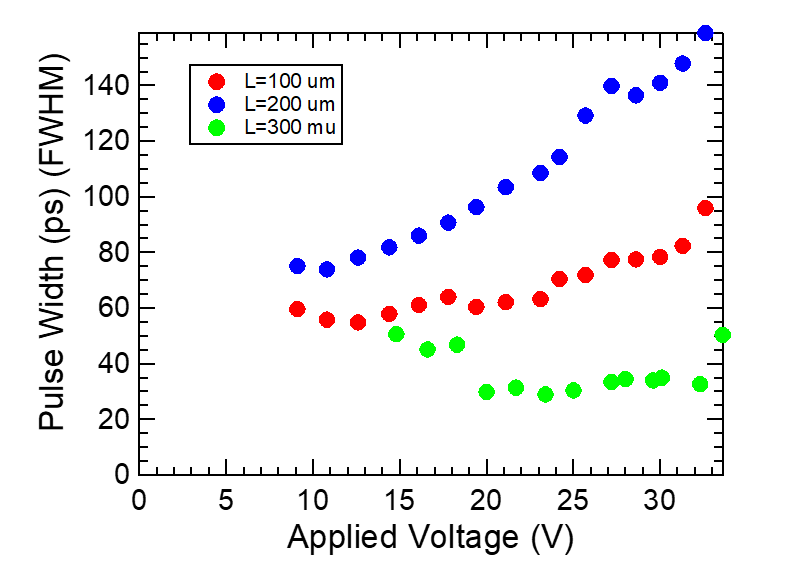
\includegraphics[width=10cm]{figure/fig_3_2_3QW_ridge_GS_FWHM.png}
		\caption{3周期歪量子井戸リッジ導波路型レーザーの光パルス幅}
		\label{fig:fig_3_2_3QW_ridge_GS_FWHM}
\end{figure}
\clearpage
\subsection{10周期歪補償量子井戸リッジ導波路型レーザーの利得スイッチング動作}%==============================
次に10周期歪補償量子井戸試料の利得スイッチング時間波形の結果を示す。

図\ref{fig:fig_3_2_10QW_ridge_L300_GS}には共振器長300 \si{\micro\metre}の結果を示す。(a)は時間波形の生データ、(b)は規格化したデータである。(a) を見ると励起強度をあげるにしたがって第1ピーク強度は大きくなっている。(b)を見ると最初はシングルピークだった光パルスが27 Vを超えたところから緩和振動がみられ複数ピークになっている。第1ピークは励起強度とともに早く立ち上がる様子が見られる。典型的な利得スイッチング動作である。
\begin{figure}[h]
	\centering
	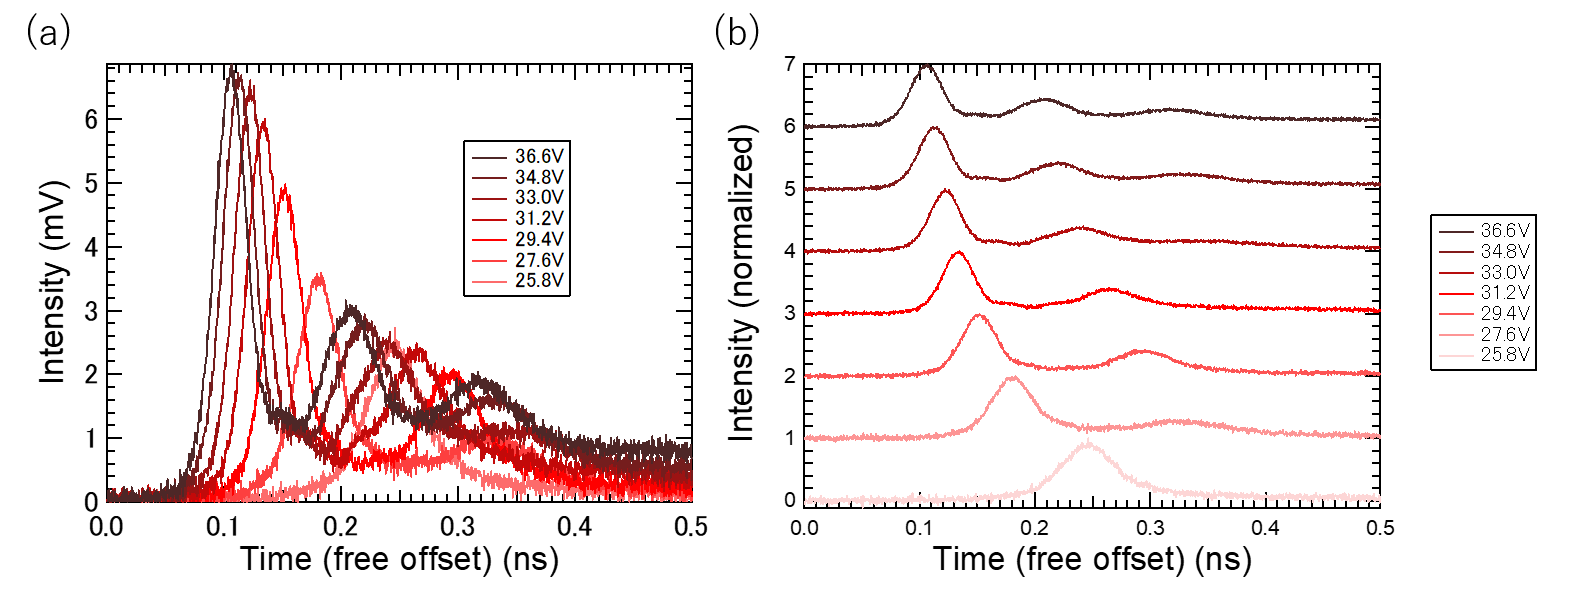
\includegraphics[width=15cm]{figure/fig_3_2_10QW_ridge_L300_GS.png}
		\caption{10周期歪補償量子井戸リッジ導波路型レーザー $L$=300 \si{\micro\metre} の利得スイッチング光パルスの時間波形}
		\label{fig:fig_3_2_10QW_ridge_L300_GS}
\end{figure}


図\ref{fig:fig_3_2_10QW_ridge_L400_GS}には共振器長$L$=400 \si{\micro\metre}の試料の結果を示す。(a)を見ると第1ピークは励起強度とともに大きくなっていく様子が見える。(b)を見ると励起強度を上げると緩和振動が見られるようになっていくことがわかる。また第1ピークの立ち上がり時間が早くなっている。
\begin{figure}[h]
	\centering
	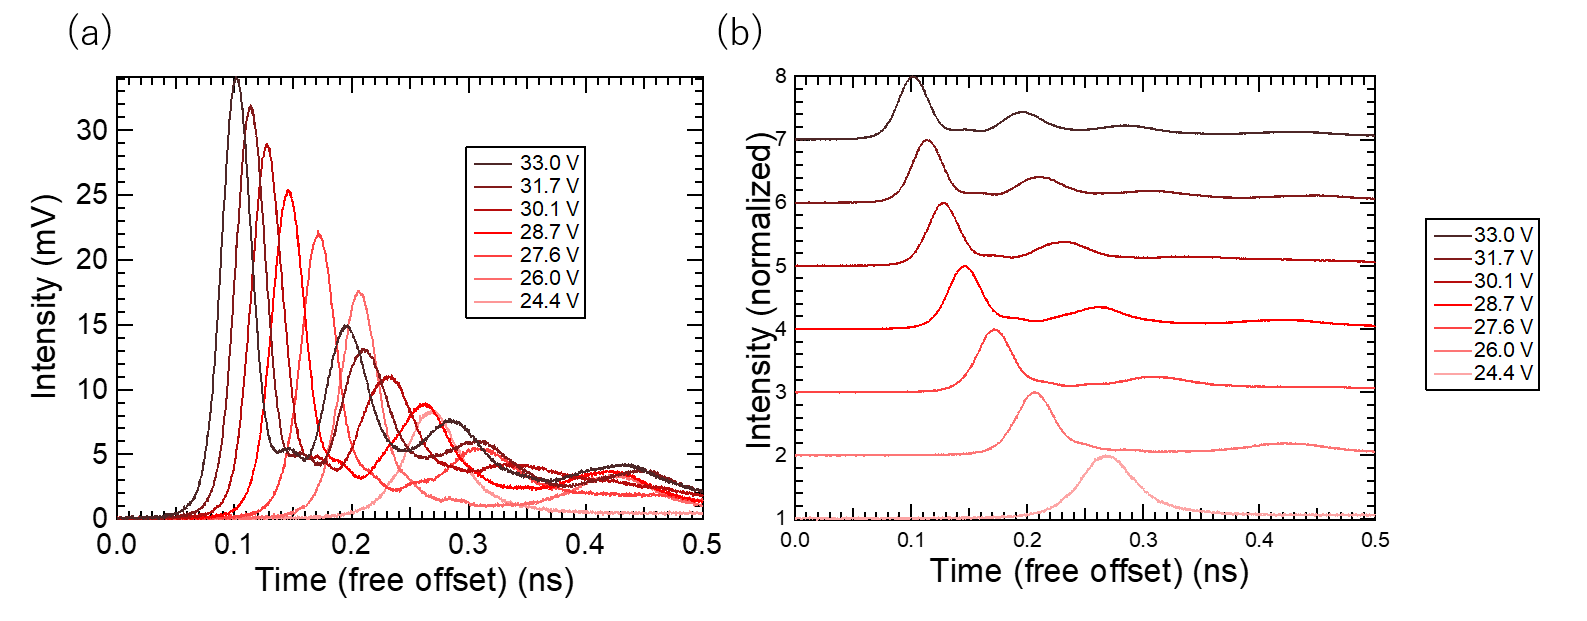
\includegraphics[width=15cm]{figure/fig_3_2_10QW_ridge_L400_GS.png}
		\caption{10歪補償量子井戸リッジ導波路型レーザー $L$=400 \si{\micro\metre} の利得スイッチング光パルスの時間波形}
		\label{fig:fig_3_2_10QW_ridge_L400_GS}
\end{figure}

%横軸の時間同じにできないの?
図\ref{fig:fig_3_2_10QW_ridge_L500_GS}に共振器長$L$=500 \si{\micro\metre}の試料の時間波形を示す。(a)を見ると第1ピークが励起強度とともに増大していくことがわかる。(b)を見ると励起強度の増大とともに立ち上がり時間が早くなっている。さらに26.6 Vを超えると緩和振動の第2パルスが見られ始める。
\begin{figure}[h]
	\centering
	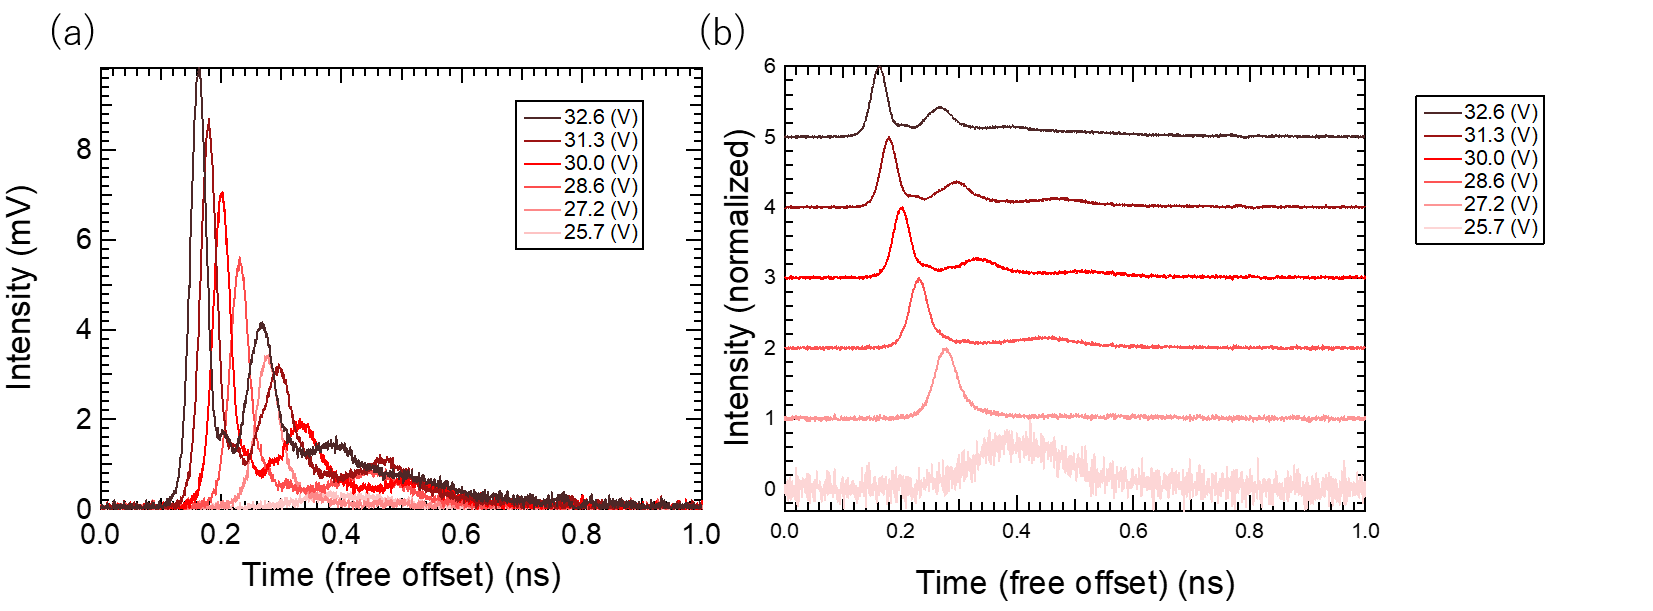
\includegraphics[width=15cm]{figure/fig_3_2_10QW_ridge_L500_GS.png}
		\caption{10周期歪補償量子井戸リッジ導波路型レーザー $L$=500 \si{\micro\metre} の利得スイッチング光パルスの時間波形}
		\label{fig:fig_3_2_10QW_ridge_L500_GS}
\end{figure}

\newpage
\subsubsection{10周期歪補償量子井戸リッジ導波路型レーザーの利得スイッチング実験のまとめ}
10周期歪補償量子井戸リッジ導波路型レーザーについてはどの全ての共振器長の試料についても典型的な利得スイッチング動作が見られた。


次図\ref{fig:fig_3_2_10QW_ridge_GS_FWHM}に10周期歪補償量子井戸リッジ導波路型レーザーの利得スイッチングパルスのパルス幅を示す。色分けは共振器長の違いを表す。
励起強度を増加していくとパルス幅は短くなる様子がどの共振器長でも見て取れる。$L$=300 \si{\micro\metre}では30 Vより強励起ではパルス幅は短くなることはなく29 ps程度で横ばいになっている。$L$=400 \si{\micro\metre}、$L$=500 \si{\micro\metre}でも印加電圧30 V付近でパルス幅の変化が小さくなっており、飽和が起きている。最短パルス幅は$L$=400 \si{\micro\metre}で26.5 psであった。共振器長依存性は見られなかった。
\begin{figure}[h]
	\centering
	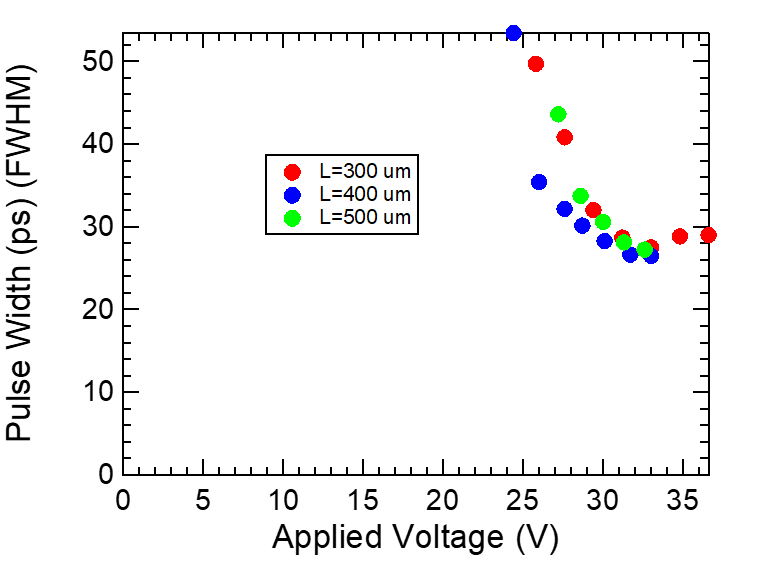
\includegraphics[width=10cm]{figure/fig_3_2_10QW_ridge_GS_FWHM.png}
		\caption{10周期歪補償量子井戸リッジ導波路型レーザーの光パルス幅}
		\label{fig:fig_3_2_10QW_ridge_GS_FWHM}
\end{figure}

\subsection{利得スイッチング実験のまとめ}%===========================

3周期歪量子井戸リッジ導波路型レーザーと10周期歪補償量子井戸リッジ導波路型レーザーについての利得スイッチング実験の結果をまとめる。


\subsubsection{3周期歪量子井戸レーザーと10周期歪補償レーザーの結果の比較}
$L$=100 \si{\micro\metre}と200 \si{\micro\metre}については試料のマウントの方法に問題があり典型的な利得スイッチングパルスは得られなかった。共振器長が$L$=300 \si{\micro\metre}試料では最短パルス幅23.4 V印加で28.9 psであった。

10周期試料については典型的な利得スイッチングパルスが得られ、最短パルス幅は$L$=400 \si{\micro\metre}で26.5 psであった。

3周期と10周期試料ではどちらも30 ps程度に収束しておりモード利得の違いによるパルス幅の差異が明確ではないと考えられる。

パルス幅を制限する外的要因として駆動電気パルスの立ち上がり時間について詳細に調べることで解明が可能であると考えられる。
\subsubsection{利得スイッチングパルスの共振器長依存性について}
先行研究によると利得スイッチングパルスの立ち下がりは共振器寿命によって決定された。
そこで式(\ref{eq:tau_p})を用いて共振器寿命を計算してみると
\begin{table}[h]
  \caption{共振器寿命}
  \label{table:table_taup}
  \centering
  \begin{tabular}{lccc}
    \hline
    試料   &  内部損失$\alpha_{int} \rm{ /cm}$&共振器長  \si{\micro\metre} &共振器寿命 $\tau_{p}$  ps \\
    \hline \hline
     3周期歪量子井戸 &   11.8 &300 &2.3\\
    10周期歪補償量子井戸  & 18.0 &300&2.01\\
    \hline
  \end{tabular}
\end{table}

計算にはR=0.3, $n_{eq}$=3.5を用いた。

実験結果はパルス幅数十psであるので共振器寿命よりも1桁大きくなっている。共振器寿命のパルス幅の決定への寄与は小さいと考えられる。共振器長を変えたときにパルス幅が変わらないことの根拠となると考えられる。

